% Options for packages loaded elsewhere
\PassOptionsToPackage{unicode}{hyperref}
\PassOptionsToPackage{hyphens}{url}
\PassOptionsToPackage{dvipsnames,svgnames,x11names}{xcolor}
%
\documentclass[
  12pt,
  letterpaper,
]{book}

\usepackage{amsmath,amssymb}
\usepackage{iftex}
\ifPDFTeX
  \usepackage[T1]{fontenc}
  \usepackage[utf8]{inputenc}
  \usepackage{textcomp} % provide euro and other symbols
\else % if luatex or xetex
  \usepackage{unicode-math}
  \defaultfontfeatures{Scale=MatchLowercase}
  \defaultfontfeatures[\rmfamily]{Ligatures=TeX,Scale=1}
\fi
\usepackage{lmodern}
\ifPDFTeX\else  
    % xetex/luatex font selection
\fi
% Use upquote if available, for straight quotes in verbatim environments
\IfFileExists{upquote.sty}{\usepackage{upquote}}{}
\IfFileExists{microtype.sty}{% use microtype if available
  \usepackage[]{microtype}
  \UseMicrotypeSet[protrusion]{basicmath} % disable protrusion for tt fonts
}{}
\makeatletter
\@ifundefined{KOMAClassName}{% if non-KOMA class
  \IfFileExists{parskip.sty}{%
    \usepackage{parskip}
  }{% else
    \setlength{\parindent}{0pt}
    \setlength{\parskip}{6pt plus 2pt minus 1pt}}
}{% if KOMA class
  \KOMAoptions{parskip=half}}
\makeatother
\usepackage{xcolor}
\usepackage[margin=1in]{geometry}
\setlength{\emergencystretch}{3em} % prevent overfull lines
\setcounter{secnumdepth}{5}
% Make \paragraph and \subparagraph free-standing
\makeatletter
\ifx\paragraph\undefined\else
  \let\oldparagraph\paragraph
  \renewcommand{\paragraph}{
    \@ifstar
      \xxxParagraphStar
      \xxxParagraphNoStar
  }
  \newcommand{\xxxParagraphStar}[1]{\oldparagraph*{#1}\mbox{}}
  \newcommand{\xxxParagraphNoStar}[1]{\oldparagraph{#1}\mbox{}}
\fi
\ifx\subparagraph\undefined\else
  \let\oldsubparagraph\subparagraph
  \renewcommand{\subparagraph}{
    \@ifstar
      \xxxSubParagraphStar
      \xxxSubParagraphNoStar
  }
  \newcommand{\xxxSubParagraphStar}[1]{\oldsubparagraph*{#1}\mbox{}}
  \newcommand{\xxxSubParagraphNoStar}[1]{\oldsubparagraph{#1}\mbox{}}
\fi
\makeatother

\usepackage{color}
\usepackage{fancyvrb}
\newcommand{\VerbBar}{|}
\newcommand{\VERB}{\Verb[commandchars=\\\{\}]}
\DefineVerbatimEnvironment{Highlighting}{Verbatim}{commandchars=\\\{\}}
% Add ',fontsize=\small' for more characters per line
\usepackage{framed}
\definecolor{shadecolor}{RGB}{241,243,245}
\newenvironment{Shaded}{\begin{snugshade}}{\end{snugshade}}
\newcommand{\AlertTok}[1]{\textcolor[rgb]{0.68,0.00,0.00}{#1}}
\newcommand{\AnnotationTok}[1]{\textcolor[rgb]{0.37,0.37,0.37}{#1}}
\newcommand{\AttributeTok}[1]{\textcolor[rgb]{0.40,0.45,0.13}{#1}}
\newcommand{\BaseNTok}[1]{\textcolor[rgb]{0.68,0.00,0.00}{#1}}
\newcommand{\BuiltInTok}[1]{\textcolor[rgb]{0.00,0.23,0.31}{#1}}
\newcommand{\CharTok}[1]{\textcolor[rgb]{0.13,0.47,0.30}{#1}}
\newcommand{\CommentTok}[1]{\textcolor[rgb]{0.37,0.37,0.37}{#1}}
\newcommand{\CommentVarTok}[1]{\textcolor[rgb]{0.37,0.37,0.37}{\textit{#1}}}
\newcommand{\ConstantTok}[1]{\textcolor[rgb]{0.56,0.35,0.01}{#1}}
\newcommand{\ControlFlowTok}[1]{\textcolor[rgb]{0.00,0.23,0.31}{\textbf{#1}}}
\newcommand{\DataTypeTok}[1]{\textcolor[rgb]{0.68,0.00,0.00}{#1}}
\newcommand{\DecValTok}[1]{\textcolor[rgb]{0.68,0.00,0.00}{#1}}
\newcommand{\DocumentationTok}[1]{\textcolor[rgb]{0.37,0.37,0.37}{\textit{#1}}}
\newcommand{\ErrorTok}[1]{\textcolor[rgb]{0.68,0.00,0.00}{#1}}
\newcommand{\ExtensionTok}[1]{\textcolor[rgb]{0.00,0.23,0.31}{#1}}
\newcommand{\FloatTok}[1]{\textcolor[rgb]{0.68,0.00,0.00}{#1}}
\newcommand{\FunctionTok}[1]{\textcolor[rgb]{0.28,0.35,0.67}{#1}}
\newcommand{\ImportTok}[1]{\textcolor[rgb]{0.00,0.46,0.62}{#1}}
\newcommand{\InformationTok}[1]{\textcolor[rgb]{0.37,0.37,0.37}{#1}}
\newcommand{\KeywordTok}[1]{\textcolor[rgb]{0.00,0.23,0.31}{\textbf{#1}}}
\newcommand{\NormalTok}[1]{\textcolor[rgb]{0.00,0.23,0.31}{#1}}
\newcommand{\OperatorTok}[1]{\textcolor[rgb]{0.37,0.37,0.37}{#1}}
\newcommand{\OtherTok}[1]{\textcolor[rgb]{0.00,0.23,0.31}{#1}}
\newcommand{\PreprocessorTok}[1]{\textcolor[rgb]{0.68,0.00,0.00}{#1}}
\newcommand{\RegionMarkerTok}[1]{\textcolor[rgb]{0.00,0.23,0.31}{#1}}
\newcommand{\SpecialCharTok}[1]{\textcolor[rgb]{0.37,0.37,0.37}{#1}}
\newcommand{\SpecialStringTok}[1]{\textcolor[rgb]{0.13,0.47,0.30}{#1}}
\newcommand{\StringTok}[1]{\textcolor[rgb]{0.13,0.47,0.30}{#1}}
\newcommand{\VariableTok}[1]{\textcolor[rgb]{0.07,0.07,0.07}{#1}}
\newcommand{\VerbatimStringTok}[1]{\textcolor[rgb]{0.13,0.47,0.30}{#1}}
\newcommand{\WarningTok}[1]{\textcolor[rgb]{0.37,0.37,0.37}{\textit{#1}}}

\providecommand{\tightlist}{%
  \setlength{\itemsep}{0pt}\setlength{\parskip}{0pt}}\usepackage{longtable,booktabs,array}
\usepackage{calc} % for calculating minipage widths
% Correct order of tables after \paragraph or \subparagraph
\usepackage{etoolbox}
\makeatletter
\patchcmd\longtable{\par}{\if@noskipsec\mbox{}\fi\par}{}{}
\makeatother
% Allow footnotes in longtable head/foot
\IfFileExists{footnotehyper.sty}{\usepackage{footnotehyper}}{\usepackage{footnote}}
\makesavenoteenv{longtable}
\usepackage{graphicx}
\makeatletter
\def\maxwidth{\ifdim\Gin@nat@width>\linewidth\linewidth\else\Gin@nat@width\fi}
\def\maxheight{\ifdim\Gin@nat@height>\textheight\textheight\else\Gin@nat@height\fi}
\makeatother
% Scale images if necessary, so that they will not overflow the page
% margins by default, and it is still possible to overwrite the defaults
% using explicit options in \includegraphics[width, height, ...]{}
\setkeys{Gin}{width=\maxwidth,height=\maxheight,keepaspectratio}
% Set default figure placement to htbp
\makeatletter
\def\fps@figure{htbp}
\makeatother
% definitions for citeproc citations
\NewDocumentCommand\citeproctext{}{}
\NewDocumentCommand\citeproc{mm}{%
  \begingroup\def\citeproctext{#2}\cite{#1}\endgroup}
\makeatletter
 % allow citations to break across lines
 \let\@cite@ofmt\@firstofone
 % avoid brackets around text for \cite:
 \def\@biblabel#1{}
 \def\@cite#1#2{{#1\if@tempswa , #2\fi}}
\makeatother
\newlength{\cslhangindent}
\setlength{\cslhangindent}{1.5em}
\newlength{\csllabelwidth}
\setlength{\csllabelwidth}{3em}
\newenvironment{CSLReferences}[2] % #1 hanging-indent, #2 entry-spacing
 {\begin{list}{}{%
  \setlength{\itemindent}{0pt}
  \setlength{\leftmargin}{0pt}
  \setlength{\parsep}{0pt}
  % turn on hanging indent if param 1 is 1
  \ifodd #1
   \setlength{\leftmargin}{\cslhangindent}
   \setlength{\itemindent}{-1\cslhangindent}
  \fi
  % set entry spacing
  \setlength{\itemsep}{#2\baselineskip}}}
 {\end{list}}
\usepackage{calc}
\newcommand{\CSLBlock}[1]{\hfill\break\parbox[t]{\linewidth}{\strut\ignorespaces#1\strut}}
\newcommand{\CSLLeftMargin}[1]{\parbox[t]{\csllabelwidth}{\strut#1\strut}}
\newcommand{\CSLRightInline}[1]{\parbox[t]{\linewidth - \csllabelwidth}{\strut#1\strut}}
\newcommand{\CSLIndent}[1]{\hspace{\cslhangindent}#1}

% header.tex
\usepackage{xcolor}        % Para colores
\usepackage{polyglossia}   % Soporte de idiomas con XeLaTeX
\setdefaultlanguage{spanish}

% Definición de colores personalizados
\definecolor{fecundidad}{HTML}{FFC125}      % Amarillo
\definecolor{supervivencia}{HTML}{36648B}   % Azul
\definecolor{crecimiento}{HTML}{548B54}     % Verde
\definecolor{retroceso}{HTML}{7A378B}       % Violeta
\definecolor{permanencia}{HTML}{26466A}     % Azul oscuro
\makeatletter
\@ifpackageloaded{caption}{}{\usepackage{caption}}
\AtBeginDocument{%
\ifdefined\contentsname
  \renewcommand*\contentsname{Table of contents}
\else
  \newcommand\contentsname{Table of contents}
\fi
\ifdefined\listfigurename
  \renewcommand*\listfigurename{List of Figures}
\else
  \newcommand\listfigurename{List of Figures}
\fi
\ifdefined\listtablename
  \renewcommand*\listtablename{List of Tables}
\else
  \newcommand\listtablename{List of Tables}
\fi
\ifdefined\figurename
  \renewcommand*\figurename{Figure}
\else
  \newcommand\figurename{Figure}
\fi
\ifdefined\tablename
  \renewcommand*\tablename{Table}
\else
  \newcommand\tablename{Table}
\fi
}
\@ifpackageloaded{float}{}{\usepackage{float}}
\floatstyle{ruled}
\@ifundefined{c@chapter}{\newfloat{codelisting}{h}{lop}}{\newfloat{codelisting}{h}{lop}[chapter]}
\floatname{codelisting}{Listing}
\newcommand*\listoflistings{\listof{codelisting}{List of Listings}}
\makeatother
\makeatletter
\makeatother
\makeatletter
\@ifpackageloaded{caption}{}{\usepackage{caption}}
\@ifpackageloaded{subcaption}{}{\usepackage{subcaption}}
\makeatother

\ifLuaTeX
  \usepackage{selnolig}  % disable illegal ligatures
\fi
\usepackage{bookmark}

\IfFileExists{xurl.sty}{\usepackage{xurl}}{} % add URL line breaks if available
\urlstyle{same} % disable monospaced font for URLs
\hypersetup{
  colorlinks=true,
  linkcolor={Maroon},
  filecolor={Maroon},
  citecolor={Blue},
  urlcolor={Blue},
  pdfcreator={LaTeX via pandoc}}


\author{}
\date{}

\begin{document}
\frontmatter

\renewcommand*\contentsname{Table of contents}
{
\hypersetup{linkcolor=}
\setcounter{tocdepth}{2}
\tableofcontents
}

\mainmatter
\chapter{El Ciclo de Vida}\label{Ciclo_Vida}

Raymond L. Tremblay

\subsubsection{Librerías de R requeridas para el siguiente
módulo}\label{libreruxedas-de-r-requeridas-para-el-siguiente-muxf3dulo}

\begin{Shaded}
\begin{Highlighting}[]
\FunctionTok{library}\NormalTok{(Rage) }\CommentTok{\# para crear diagramas de ciclo de vida y métricas de historia de vida }
\FunctionTok{library}\NormalTok{(rsvg) }\CommentTok{\# trabajar con imágenes }
\FunctionTok{library}\NormalTok{(tidyverse)}

\CommentTok{\#devtools::install\_github("rich{-}iannone/DiagrammeR") \# Instalar directamente de github para tener la versión más reciente}

\FunctionTok{library}\NormalTok{(DiagrammeR) }\CommentTok{\# para crear diagramas de ciclo de vida}
\end{Highlighting}
\end{Shaded}

\section{Introducción}\label{introducciuxf3n}

Todas las especies biológicas poseen una historia de vida que comienza
con el nacimiento y culmina con la muerte. En su hábitat natural, la
supervivencia de la mayoría de las plantas depende de la continuidad de
todas las etapas de desarrollo ---semilla, plántula, juvenil, adulto y
eventos reproductivos--- a lo largo del ciclo vital. Aunque estas etapas
suelen incluirse en los análisis, algunas pueden omitirse; por ejemplo,
la fase de semilla en especies que se reproducen vegetativamente
mediante clones (como plátanos, papas, piñas, vainillas y numerosas
plantas ornamentales y medicinales).

Desde la perspectiva de la conservación y la ecología, es fundamental
evaluar el ciclo de vida completo, identificar las características que
limitan la supervivencia y la reproducción en el hábitat natural, y
determinar cuáles etapas son más relevantes para el crecimiento
poblacional. La persistencia de una especie depende de procesos viables
que mantengan una población estable o en aumento. El método más adecuado
para evaluar esta persistencia consiste en analizar las etapas críticas
de la historia de vida y aplicar matrices de proyección poblacional para
estimar los cambios en el tiempo, identificando si la población crece,
disminuye o se mantiene estable.

Antes de iniciar cualquier estudio poblacional, se recomienda elaborar
un diagrama del ciclo de vida de la especie de interés. Este paso previo
a la recolección de datos permite visualizar el ciclo hipotético,
identificar etapas críticas, factores que influyen en el crecimiento y
supervivencia, y definir qué información debe obtenerse en campo. Los
diagramas son herramientas esenciales para comprender la biología del
organismo y anticipar los factores que afectan su desarrollo.

Un diagrama de ciclo de vida es una representación gráfica de los
estadios que atraviesa un organismo a lo largo de su existencia. En este
capítulo, se mostrará cómo crear diagramas de ciclo de vida en
\texttt{R} utilizando la librería \texttt{Rage}, enfatizando la
diferencia entre el modelo hipotético y los datos que pueden
recolectarse en campo.

\begin{center}\rule{0.5\linewidth}{0.5pt}\end{center}

\section{Ejemplo de ciclos de vida
sencillo}\label{ejemplo-de-ciclos-de-vida-sencillo}

En este primer ejemplo se presenta un ciclo de vida simple con tres
estados: semillas, plántulas y adultos. Supongamos que se trata de una
planta que se reproduce sexualmente y cuyas semillas no forman un banco,
lo que implica que no hay latencia y germinan en el mismo año en que son
dispersadas. En este escenario, las semillas germinan y se convierten en
plántulas o mueren; las plántulas crecen y se transforman en adultos o
mueren; y los adultos se reproducen y finalmente mueren. Cada etapa dura
un año: el primero corresponde a la semilla, el segundo a la plántula y
el tercero al adulto, que contribuye con nuevas semillas. Por lo tanto,
el ciclo completo dura tres años. Este es un ejemplo hipotético, ya que
en la naturaleza los organismos rara vez presentan ciclos tan simples.

La matriz de transición para este ciclo es la siguiente: el 50 \% de las
semillas germinan y se convierten en plántulas, el 40 \% de las
plántulas alcanzan la etapa adulta y cada adulto produce en promedio 3.2
semillas. En el diagrama, las líneas verdes representan crecimiento y
las líneas amarillas representan reproducción.

\begin{Shaded}
\begin{Highlighting}[]
\NormalTok{matA }\OtherTok{\textless{}{-}} \FunctionTok{rbind}\NormalTok{(}
  \FunctionTok{c}\NormalTok{(}\FloatTok{0.0}\NormalTok{, }\FloatTok{0.0}\NormalTok{, }\FloatTok{3.2}\NormalTok{),}
  \FunctionTok{c}\NormalTok{(}\FloatTok{0.5}\NormalTok{, }\FloatTok{0.0}\NormalTok{, }\FloatTok{0.0}\NormalTok{),}
  \FunctionTok{c}\NormalTok{(}\FloatTok{0.0}\NormalTok{, }\FloatTok{0.4}\NormalTok{, }\FloatTok{0.0}\NormalTok{)}
\NormalTok{)}


\NormalTok{etapas }\OtherTok{\textless{}{-}} \FunctionTok{c}\NormalTok{(}\StringTok{"semillas"}\NormalTok{, }\StringTok{"plantulas"}\NormalTok{, }\StringTok{"adultos"}\NormalTok{)}
\NormalTok{title }\OtherTok{\textless{}{-}} \StringTok{"Especie hipotética"} \CommentTok{\# si no quiere titulo, pon title \textless{}{-} NULL}
\NormalTok{graph }\OtherTok{\textless{}{-}} \FunctionTok{expand.grid}\NormalTok{(}\AttributeTok{to =}\NormalTok{ etapas, }\AttributeTok{from =}\NormalTok{ etapas)}
\NormalTok{graph}\SpecialCharTok{$}\NormalTok{trans }\OtherTok{\textless{}{-}} \FunctionTok{round}\NormalTok{(}\FunctionTok{c}\NormalTok{(matA), }\DecValTok{3}\NormalTok{)}
\NormalTok{graph }\OtherTok{\textless{}{-}}\NormalTok{ graph[graph}\SpecialCharTok{$}\NormalTok{trans }\SpecialCharTok{\textgreater{}} \DecValTok{0}\NormalTok{, ]}
\NormalTok{nodes }\OtherTok{\textless{}{-}} \FunctionTok{paste}\NormalTok{(}\FunctionTok{paste0}\NormalTok{(}\StringTok{"\textquotesingle{}"}\NormalTok{, etapas, }\StringTok{"\textquotesingle{}"}\NormalTok{), }\AttributeTok{collapse =} \StringTok{"; "}\NormalTok{)}
\NormalTok{graph}\SpecialCharTok{$}\NormalTok{min\_len }\OtherTok{\textless{}{-}}\NormalTok{ (}\FunctionTok{as.numeric}\NormalTok{(graph}\SpecialCharTok{$}\NormalTok{to) }\SpecialCharTok{{-}} \FunctionTok{as.numeric}\NormalTok{(graph}\SpecialCharTok{$}\NormalTok{from)) }\SpecialCharTok{*} \DecValTok{3}
\NormalTok{graph}\SpecialCharTok{$}\NormalTok{col }\OtherTok{\textless{}{-}} \FunctionTok{c}\NormalTok{(}
  \StringTok{"PaleGreen4"}\NormalTok{, }\StringTok{"PaleGreen4"}\NormalTok{, }\StringTok{"Goldenrod1"}
\NormalTok{)}
\NormalTok{edges }\OtherTok{\textless{}{-}} \FunctionTok{paste0}\NormalTok{(}\StringTok{"\textquotesingle{}"}\NormalTok{, graph}\SpecialCharTok{$}\NormalTok{from, }\StringTok{"\textquotesingle{}"}\NormalTok{, }\StringTok{" {-}\textgreater{} "}\NormalTok{, }\StringTok{"\textquotesingle{}"}\NormalTok{, graph}\SpecialCharTok{$}\NormalTok{to, }\StringTok{"\textquotesingle{}"}\NormalTok{,}
  \StringTok{"[minlen="}\NormalTok{, graph}\SpecialCharTok{$}\NormalTok{min\_len,}
  \StringTok{",fontsize="}\NormalTok{, }\DecValTok{10}\NormalTok{,}
  \StringTok{",color="}\NormalTok{, graph}\SpecialCharTok{$}\NormalTok{col,}
  \StringTok{",xlabel="}\NormalTok{, }\FunctionTok{paste}\NormalTok{(}\StringTok{"}\SpecialCharTok{\textbackslash{}"}\StringTok{"}\NormalTok{, graph}\SpecialCharTok{$}\NormalTok{trans),}
  \StringTok{"}\SpecialCharTok{\textbackslash{}"}\StringTok{]}\SpecialCharTok{\textbackslash{}n}\StringTok{"}\NormalTok{,}
  \AttributeTok{collapse =} \StringTok{""}
\NormalTok{)}
\FunctionTok{grViz}\NormalTok{(}
  \FunctionTok{paste}\NormalTok{(}
    \StringTok{"}
\StringTok{digraph \{}
\StringTok{  \{}
\StringTok{    graph[overlap=false];}
\StringTok{    rank=same;}
\StringTok{    node [shape="}\NormalTok{, }\StringTok{"egg"}\NormalTok{, }\StringTok{", fontsize="}\NormalTok{, }\DecValTok{12}\NormalTok{, }\StringTok{"];"}\NormalTok{,}
\NormalTok{    nodes, }\StringTok{"}
\StringTok{  \}"}\NormalTok{,}
    \StringTok{"ordering=out}
\StringTok{  x [style=invis]}
\StringTok{  x {-}\textgreater{} \{"}\NormalTok{, nodes, }\StringTok{"\} [style=invis]"}\NormalTok{, edges,}
    \StringTok{"labelloc=}\SpecialCharTok{\textbackslash{}"}\StringTok{t}\SpecialCharTok{\textbackslash{}"}\StringTok{;}
\StringTok{  label=}\SpecialCharTok{\textbackslash{}"}\StringTok{"}\NormalTok{, title, }\StringTok{"}\SpecialCharTok{\textbackslash{}"}
\StringTok{\}"}
\NormalTok{  )}
\NormalTok{)  }\CommentTok{\# \%\textgreater{}\%}
\end{Highlighting}
\end{Shaded}

\begin{verbatim}
file:////private/var/folders/3k/1ft37x9130vdbz21tw1497x40000gn/T/RtmpTIXuwN/file1061a31d6c01f/widget1061a9df4cc9.html screenshot completed
\end{verbatim}

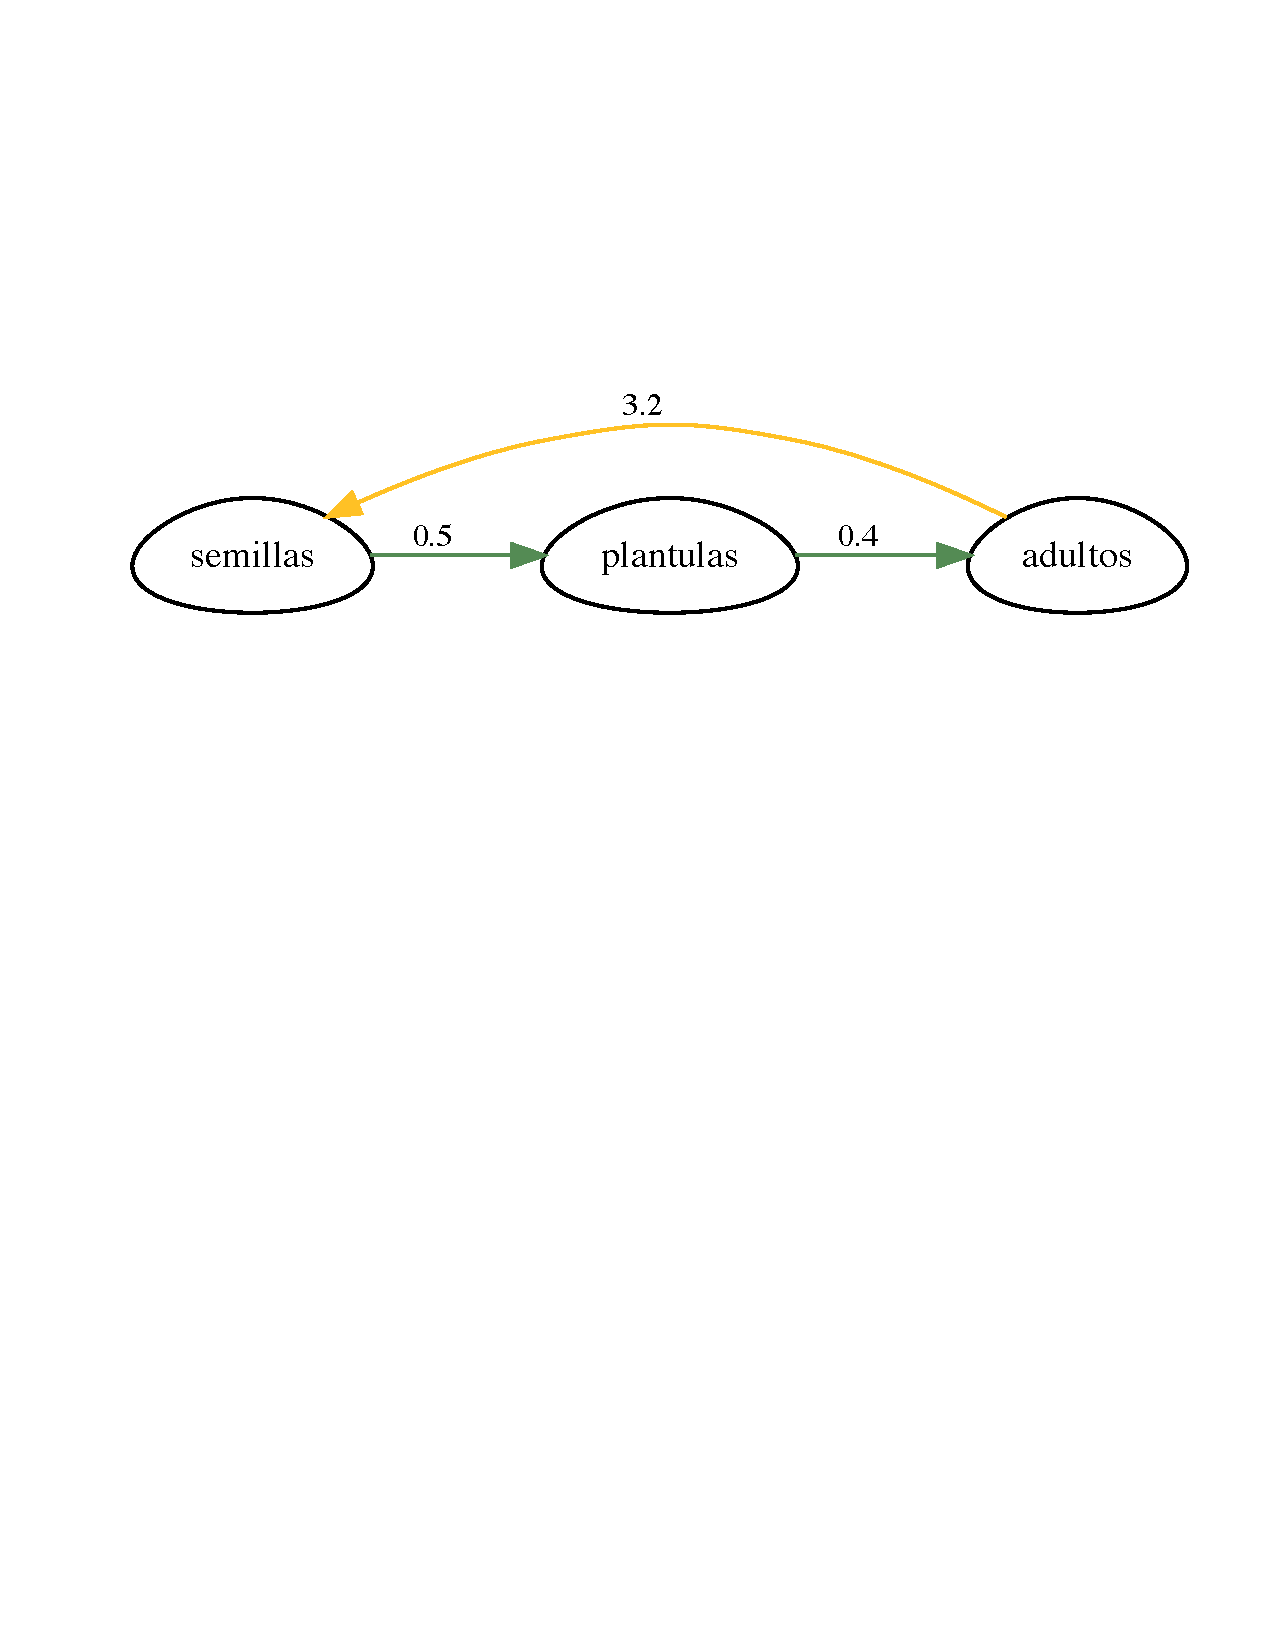
\includegraphics{103-Ciclos_de_Vida_files/figure-pdf/CV_2-1.pdf}

\begin{Shaded}
\begin{Highlighting}[]
   \CommentTok{\# export\_svg \%\textgreater{}\% charToRaw \%\textgreater{}\% rsvg\_png("graph.png")}
\end{Highlighting}
\end{Shaded}

\begin{center}\rule{0.5\linewidth}{0.5pt}\end{center}

\section{Ejemplo de una orquídea
hipotética}\label{ejemplo-de-una-orquuxeddea-hipotuxe9tica}

El ciclo de vida hipotético de una orquídea epífita se representa en el
gráfico mediante líneas verdes para indicar transición entre etapas,
líneas rojas para señalar permanencia y líneas amarillas para la
reproducción. El ciclo comienza con la germinación de la semilla sobre
la corteza de un árbol, seguida por las fases de plántula, juvenil y
adulto, etapa en la cual ocurre la floración y producción de semillas.
Exceptuando la fase de semilla, cada etapa puede prolongarse de un año a
otro, lo que evidencia un ciclo plurianual; esta característica se
refleja en la diagonal principal de la matriz de transición, cuyos
valores son mayores a cero cuando existe permanencia. Solo los
individuos adultos son capaces de reproducirse. Si el diagrama
correspondiera a datos empíricos, sería necesario contar con información
para todas las etapas (semilla, plántula, juvenil y adulto); sin
embargo, la revisión bibliográfica realizada no identificó estudios que
incluyan datos completos, debido principalmente a la dificultad de
localizar semillas y plántulas en condiciones naturales, dado su tamaño
extremadamente reducido (milimétrico) y la complejidad de seguir su
desarrollo a lo largo del tiempo.

\begin{Shaded}
\begin{Highlighting}[]
\CommentTok{\# hidden code to produce figures}
\NormalTok{matA\_ho }\OtherTok{\textless{}{-}} \FunctionTok{rbind}\NormalTok{(}
  \FunctionTok{c}\NormalTok{(}\FloatTok{0.0}\NormalTok{, }\FloatTok{0.0}\NormalTok{, }\FloatTok{0.0}\NormalTok{, }\FloatTok{3.2}\NormalTok{),}
  \FunctionTok{c}\NormalTok{(}\FloatTok{0.5}\NormalTok{, }\FloatTok{0.3}\NormalTok{, }\FloatTok{0.0}\NormalTok{, }\FloatTok{0.0}\NormalTok{),}
  \FunctionTok{c}\NormalTok{(}\FloatTok{0.0}\NormalTok{, }\FloatTok{0.4}\NormalTok{, }\FloatTok{0.20}\NormalTok{, }\FloatTok{0.0}\NormalTok{),}
  \FunctionTok{c}\NormalTok{(}\FloatTok{0.0}\NormalTok{, }\FloatTok{0.0}\NormalTok{, }\FloatTok{0.40}\NormalTok{, }\FloatTok{0.80}\NormalTok{)}
\NormalTok{)}


\NormalTok{etapas\_ho }\OtherTok{\textless{}{-}} \FunctionTok{c}\NormalTok{(}\StringTok{"semillas"}\NormalTok{, }\StringTok{"plantulas"}\NormalTok{, }\StringTok{"juvenil"}\NormalTok{, }\StringTok{"adultos"}\NormalTok{)}
\NormalTok{title }\OtherTok{\textless{}{-}} \ConstantTok{NULL}
\NormalTok{graph }\OtherTok{\textless{}{-}} \FunctionTok{expand.grid}\NormalTok{(}\AttributeTok{to =}\NormalTok{ etapas\_ho, }\AttributeTok{from =}\NormalTok{ etapas\_ho)}
\NormalTok{graph}\SpecialCharTok{$}\NormalTok{trans }\OtherTok{\textless{}{-}} \FunctionTok{round}\NormalTok{(}\FunctionTok{c}\NormalTok{(matA\_ho), }\DecValTok{3}\NormalTok{)}
\NormalTok{graph }\OtherTok{\textless{}{-}}\NormalTok{ graph[graph}\SpecialCharTok{$}\NormalTok{trans }\SpecialCharTok{\textgreater{}} \DecValTok{0}\NormalTok{, ]}
\NormalTok{nodes }\OtherTok{\textless{}{-}} \FunctionTok{paste}\NormalTok{(}\FunctionTok{paste0}\NormalTok{(}\StringTok{"\textquotesingle{}"}\NormalTok{, etapas\_ho, }\StringTok{"\textquotesingle{}"}\NormalTok{), }\AttributeTok{collapse =} \StringTok{"; "}\NormalTok{)}
\NormalTok{graph}\SpecialCharTok{$}\NormalTok{min\_len }\OtherTok{\textless{}{-}}\NormalTok{ (}\FunctionTok{as.numeric}\NormalTok{(graph}\SpecialCharTok{$}\NormalTok{to) }\SpecialCharTok{{-}} \FunctionTok{as.numeric}\NormalTok{(graph}\SpecialCharTok{$}\NormalTok{from)) }\SpecialCharTok{*} \DecValTok{3}
\NormalTok{graph}\SpecialCharTok{$}\NormalTok{col }\OtherTok{\textless{}{-}} \FunctionTok{c}\NormalTok{(}
  \StringTok{"PaleGreen4"}\NormalTok{, }
  \StringTok{"red"}\NormalTok{, }\StringTok{"PaleGreen4"}\NormalTok{, }
  \StringTok{"red"}\NormalTok{, }\StringTok{"PaleGreen4"}\NormalTok{, }
  \StringTok{"Goldenrod1"}\NormalTok{, }\StringTok{"red"}
\NormalTok{)}
\NormalTok{edges }\OtherTok{\textless{}{-}} \FunctionTok{paste0}\NormalTok{(}\StringTok{"\textquotesingle{}"}\NormalTok{, graph}\SpecialCharTok{$}\NormalTok{from, }\StringTok{"\textquotesingle{}"}\NormalTok{, }\StringTok{" {-}\textgreater{} "}\NormalTok{, }\StringTok{"\textquotesingle{}"}\NormalTok{, graph}\SpecialCharTok{$}\NormalTok{to, }\StringTok{"\textquotesingle{}"}\NormalTok{,}
  \StringTok{"[minlen="}\NormalTok{, graph}\SpecialCharTok{$}\NormalTok{min\_len,}
  \StringTok{",fontsize="}\NormalTok{, }\DecValTok{10}\NormalTok{,}
  \StringTok{",color="}\NormalTok{, graph}\SpecialCharTok{$}\NormalTok{col,}
  \StringTok{",xlabel="}\NormalTok{, }\FunctionTok{paste}\NormalTok{(}\StringTok{"}\SpecialCharTok{\textbackslash{}"}\StringTok{"}\NormalTok{, graph}\SpecialCharTok{$}\NormalTok{trans),}
  \StringTok{"}\SpecialCharTok{\textbackslash{}"}\StringTok{]}\SpecialCharTok{\textbackslash{}n}\StringTok{"}\NormalTok{,}
  \AttributeTok{collapse =} \StringTok{""}
\NormalTok{)}
\FunctionTok{grViz}\NormalTok{(}
  \FunctionTok{paste}\NormalTok{(}
    \StringTok{"}
\StringTok{digraph \{}
\StringTok{  \{}
\StringTok{    graph[overlap=false];}
\StringTok{    rank=same;}
\StringTok{    node [shape="}\NormalTok{, }\StringTok{"egg"}\NormalTok{, }\StringTok{", fontsize="}\NormalTok{, }\DecValTok{12}\NormalTok{, }\StringTok{"];"}\NormalTok{,}
\NormalTok{    nodes, }\StringTok{"}
\StringTok{  \}"}\NormalTok{,}
    \StringTok{"ordering=out}
\StringTok{  x [style=invis]}
\StringTok{  x {-}\textgreater{} \{"}\NormalTok{, nodes, }\StringTok{"\} [style=invis]"}\NormalTok{, edges,}
    \StringTok{"labelloc=}\SpecialCharTok{\textbackslash{}"}\StringTok{t}\SpecialCharTok{\textbackslash{}"}\StringTok{;}
\StringTok{  label=}\SpecialCharTok{\textbackslash{}"}\StringTok{"}\NormalTok{, title, }\StringTok{"}\SpecialCharTok{\textbackslash{}"}
\StringTok{\}"}
\NormalTok{  )}
\NormalTok{) }
\end{Highlighting}
\end{Shaded}

\begin{verbatim}
file:////private/var/folders/3k/1ft37x9130vdbz21tw1497x40000gn/T/RtmpTIXuwN/file1061a409c8c3/widget1061a1e5b7c47.html screenshot completed
\end{verbatim}

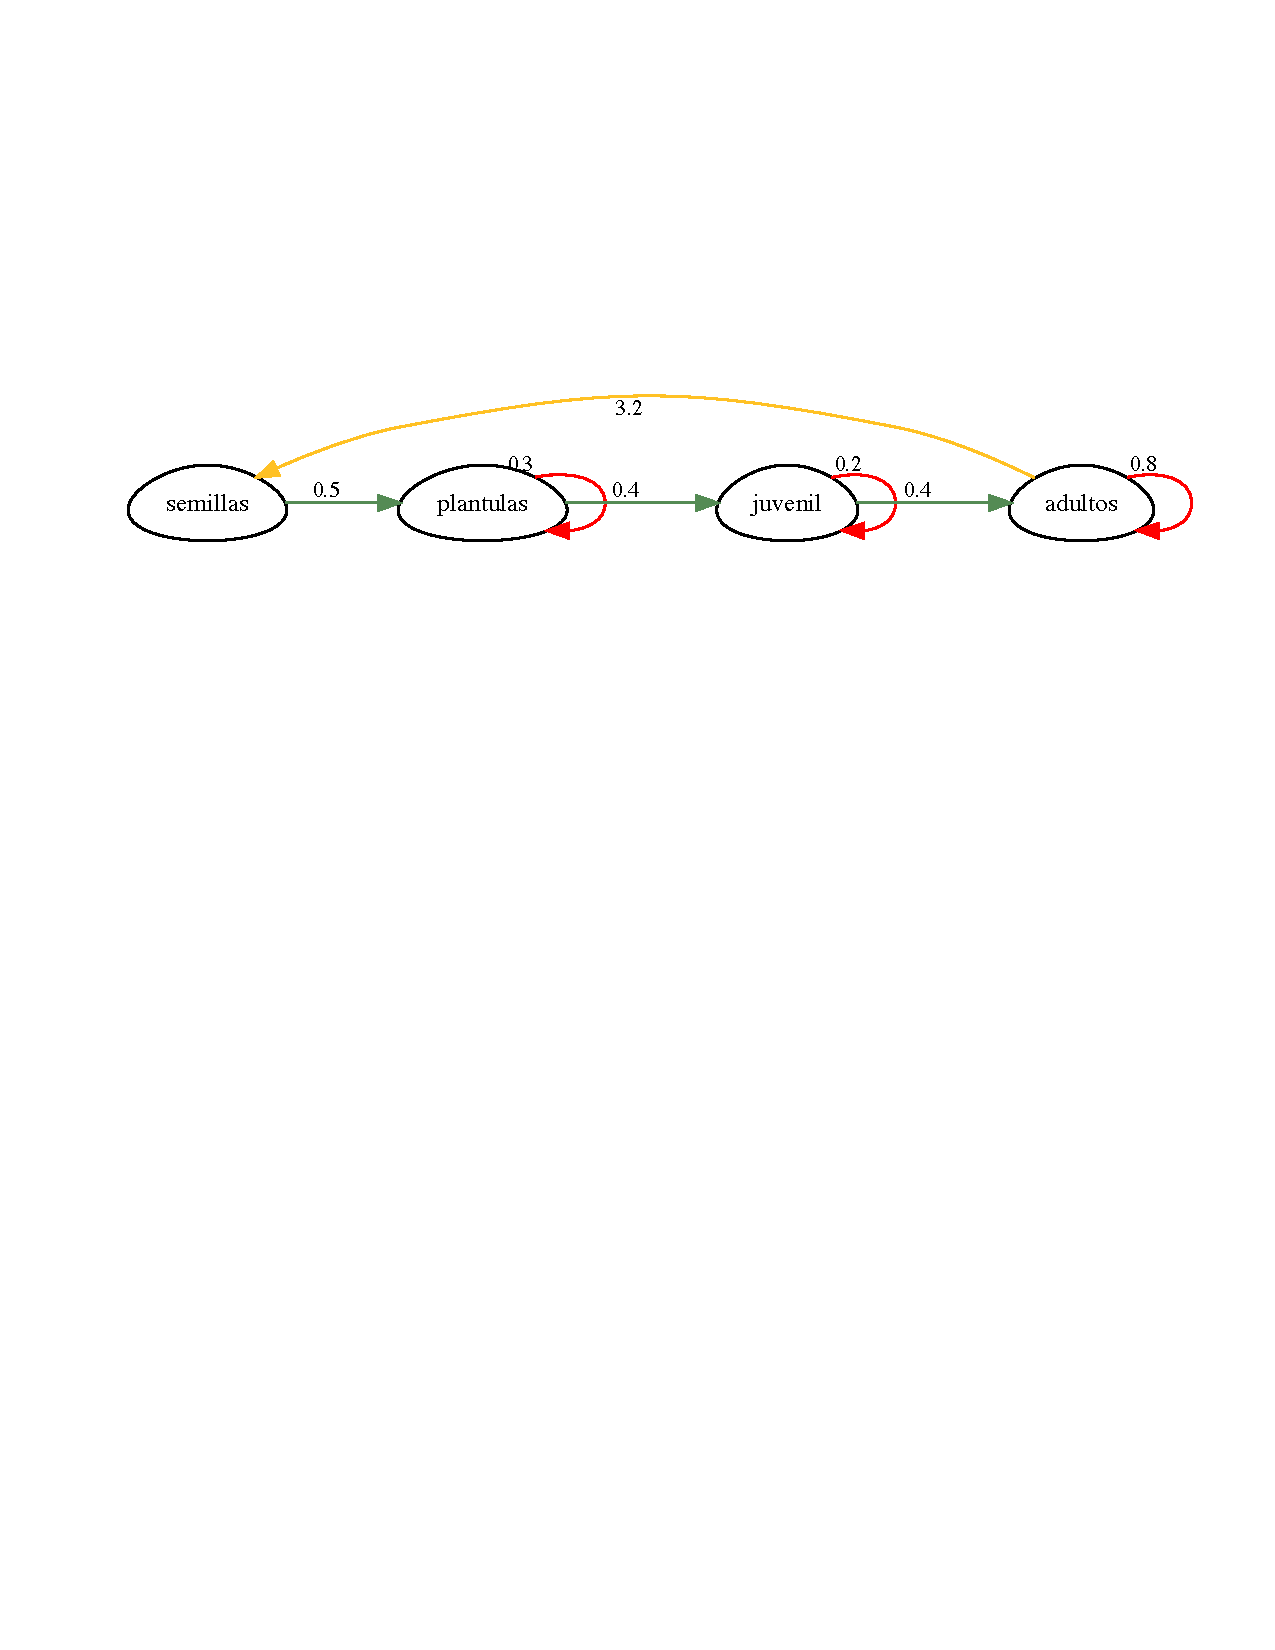
\includegraphics{103-Ciclos_de_Vida_files/figure-pdf/CV_3-1.pdf}

\begin{center}\rule{0.5\linewidth}{0.5pt}\end{center}

\section{Ciclo de vida de orquídeas en la literatura
científica}\label{ciclo-de-vida-de-orquuxeddeas-en-la-literatura-cientuxedfica}

A continuación se presentan diversos esquemas de ciclo de vida
utilizados en distintas publicaciones. Estos ejemplos evidencian la
ausencia de un modelo estandarizado, ya que cada investigador define un
ciclo particular en función de su comprensión del ciclo biológico de la
especie estudiada, la factibilidad de seguimiento de individuos a lo
largo del tiempo y los objetivos específicos de la investigación.

Los casos analizados incluyen tanto especies terrestres como epífitas, y
reflejan la diferencia entre los ciclos de vida hipotéticos y las
limitaciones impuestas por la recolección de datos en condiciones de
campo. Esta variabilidad pone de manifiesto la complejidad inherente al
estudio demográfico de orquídeas y la necesidad de adaptar los modelos a
las características ecológicas y metodológicas de cada estudio.

\subsection{Especies Epífitas}\label{especies-epuxedfitas}

\subsubsection{\texorpdfstring{\emph{Laelia
speciosa}}{Laelia speciosa}}\label{laelia-speciosa}

La información presentada se basa en la tesina de Mariana
Hernández-Apolinar (Hernández-Apolinar, 1992), uno de los primeros
estudios sobre dinámica poblacional en orquídeas epífitas. El objetivo
principal de dicho trabajo fue evaluar el impacto de la recolección
sobre la dinámica poblacional de \emph{Laelia speciosa}.

El ciclo de vida propuesto se compone de cinco etapas, según lo
ilustrado en la figura 25a de la tesina:

\begin{itemize}
\tightlist
\item
  Semillas
\item
  Plántulas
\item
  3 etapas de tamaño de planta donde 2 de las etapas son adultos y
  pueden producir semillas
\end{itemize}

Es importante señalar que se realizó una estimación tanto de la cantidad
de semillas producidas como de la proporción que germina y se convierte
en plántula en el ciclo siguiente. Este enfoque permitió incorporar
procesos de transición y reproducción en el modelo, a pesar de las
limitaciones inherentes a la observación directa de semillas y plántulas
en condiciones naturales.

\begin{Shaded}
\begin{Highlighting}[]
\NormalTok{matA\_Ls }\OtherTok{\textless{}{-}} \FunctionTok{rbind}\NormalTok{(}
  \FunctionTok{c}\NormalTok{(}\FloatTok{0.0}\NormalTok{, }\FloatTok{0.0}\NormalTok{, }\FloatTok{0.00}\NormalTok{, }\DecValTok{52686}\NormalTok{, }\DecValTok{127324}\NormalTok{),}
  \FunctionTok{c}\NormalTok{(}\FloatTok{0.00022}\NormalTok{, }\FloatTok{0.0}\NormalTok{, }\FloatTok{0.00}\NormalTok{, }\FloatTok{0.0}\NormalTok{, }\FloatTok{0.0}\NormalTok{),}
  \FunctionTok{c}\NormalTok{(}\FloatTok{0.0}\NormalTok{, }\FloatTok{0.71}\NormalTok{, }\FloatTok{0.93}\NormalTok{, }\FloatTok{0.0}\NormalTok{, }\FloatTok{0.0}\NormalTok{),}
  \FunctionTok{c}\NormalTok{(}\FloatTok{0.0}\NormalTok{, }\FloatTok{0.0}\NormalTok{, }\FloatTok{0.07}\NormalTok{, }\FloatTok{0.76}\NormalTok{, }\FloatTok{0.0}\NormalTok{),}
  \FunctionTok{c}\NormalTok{(}\FloatTok{0.0}\NormalTok{, }\FloatTok{0.0}\NormalTok{, }\FloatTok{0.00}\NormalTok{, }\FloatTok{0.24}\NormalTok{, }\FloatTok{0.75}\NormalTok{)}
\NormalTok{)}


\NormalTok{etapas\_Ls }\OtherTok{\textless{}{-}} \FunctionTok{c}\NormalTok{(}\StringTok{"semillas"}\NormalTok{, }\StringTok{"plántulas"}\NormalTok{, }\StringTok{"adulto 1"}\NormalTok{, }\StringTok{"adulto 2"}\NormalTok{, }\StringTok{"adulto 3"}\NormalTok{)}
\NormalTok{title }\OtherTok{\textless{}{-}} \ConstantTok{NULL}
\NormalTok{graph }\OtherTok{\textless{}{-}} \FunctionTok{expand.grid}\NormalTok{(}\AttributeTok{to =}\NormalTok{ etapas\_Ls, }\AttributeTok{from =}\NormalTok{ etapas\_Ls)}
\NormalTok{graph}\SpecialCharTok{$}\NormalTok{trans }\OtherTok{\textless{}{-}} \FunctionTok{round}\NormalTok{(}\FunctionTok{c}\NormalTok{(matA\_Ls), }\DecValTok{5}\NormalTok{)}
\NormalTok{graph }\OtherTok{\textless{}{-}}\NormalTok{ graph[graph}\SpecialCharTok{$}\NormalTok{trans }\SpecialCharTok{\textgreater{}} \DecValTok{0}\NormalTok{, ]}
\NormalTok{nodes }\OtherTok{\textless{}{-}} \FunctionTok{paste}\NormalTok{(}\FunctionTok{paste0}\NormalTok{(}\StringTok{"\textquotesingle{}"}\NormalTok{, etapas\_Ls, }\StringTok{"\textquotesingle{}"}\NormalTok{), }\AttributeTok{collapse =} \StringTok{"; "}\NormalTok{)}
\NormalTok{graph}\SpecialCharTok{$}\NormalTok{min\_len }\OtherTok{\textless{}{-}}\NormalTok{ (}\FunctionTok{as.numeric}\NormalTok{(graph}\SpecialCharTok{$}\NormalTok{to) }\SpecialCharTok{{-}} \FunctionTok{as.numeric}\NormalTok{(graph}\SpecialCharTok{$}\NormalTok{from)) }\SpecialCharTok{*} \DecValTok{3}
\NormalTok{graph}\SpecialCharTok{$}\NormalTok{col }\OtherTok{\textless{}{-}} \FunctionTok{c}\NormalTok{(}
  \StringTok{"PaleGreen4"}\NormalTok{, }
  \StringTok{"PaleGreen4"}\NormalTok{, }
  \StringTok{"red"}\NormalTok{, }\StringTok{"PaleGreen4"}\NormalTok{, }
  \StringTok{"Goldenrod1"}\NormalTok{, }\StringTok{"red"}\NormalTok{, }\StringTok{"PaleGreen4"}\NormalTok{,}
  \StringTok{"Goldenrod1"}\NormalTok{, }\StringTok{"red"}
\NormalTok{)}
\NormalTok{edges }\OtherTok{\textless{}{-}} \FunctionTok{paste0}\NormalTok{(}\StringTok{"\textquotesingle{}"}\NormalTok{, graph}\SpecialCharTok{$}\NormalTok{from, }\StringTok{"\textquotesingle{}"}\NormalTok{, }\StringTok{" {-}\textgreater{} "}\NormalTok{, }\StringTok{"\textquotesingle{}"}\NormalTok{, graph}\SpecialCharTok{$}\NormalTok{to, }\StringTok{"\textquotesingle{}"}\NormalTok{,}
  \StringTok{"[minlen="}\NormalTok{, graph}\SpecialCharTok{$}\NormalTok{min\_len,}
  \StringTok{",fontsize="}\NormalTok{, }\DecValTok{10}\NormalTok{,}
  \StringTok{",color="}\NormalTok{, graph}\SpecialCharTok{$}\NormalTok{col,}
  \StringTok{",xlabel="}\NormalTok{, }\FunctionTok{paste}\NormalTok{(}\StringTok{"}\SpecialCharTok{\textbackslash{}"}\StringTok{"}\NormalTok{, graph}\SpecialCharTok{$}\NormalTok{trans),}
  \StringTok{"}\SpecialCharTok{\textbackslash{}"}\StringTok{]}\SpecialCharTok{\textbackslash{}n}\StringTok{"}\NormalTok{,}
  \AttributeTok{collapse =} \StringTok{""}
\NormalTok{)}
\FunctionTok{grViz}\NormalTok{(}
  \FunctionTok{paste}\NormalTok{(}
    \StringTok{"}
\StringTok{digraph \{}
\StringTok{  \{}
\StringTok{    graph[overlap=false];}
\StringTok{    rank=same;}
\StringTok{    node [shape="}\NormalTok{, }\StringTok{"egg"}\NormalTok{, }\StringTok{", fontsize="}\NormalTok{, }\DecValTok{12}\NormalTok{, }\StringTok{"];"}\NormalTok{,}
\NormalTok{    nodes, }\StringTok{"}
\StringTok{  \}"}\NormalTok{,}
    \StringTok{"ordering=out}
\StringTok{  x [style=invis]}
\StringTok{  x {-}\textgreater{} \{"}\NormalTok{, nodes, }\StringTok{"\} [style=invis]"}\NormalTok{, edges,}
    \StringTok{"labelloc=}\SpecialCharTok{\textbackslash{}"}\StringTok{t}\SpecialCharTok{\textbackslash{}"}\StringTok{;}
\StringTok{  label=}\SpecialCharTok{\textbackslash{}"}\StringTok{"}\NormalTok{, title, }\StringTok{"}\SpecialCharTok{\textbackslash{}"}
\StringTok{\}"}
\NormalTok{  )}
\NormalTok{) }
\end{Highlighting}
\end{Shaded}

\begin{verbatim}
file:////private/var/folders/3k/1ft37x9130vdbz21tw1497x40000gn/T/RtmpTIXuwN/file1061a46f51c36/widget1061a60f419f.html screenshot completed
\end{verbatim}

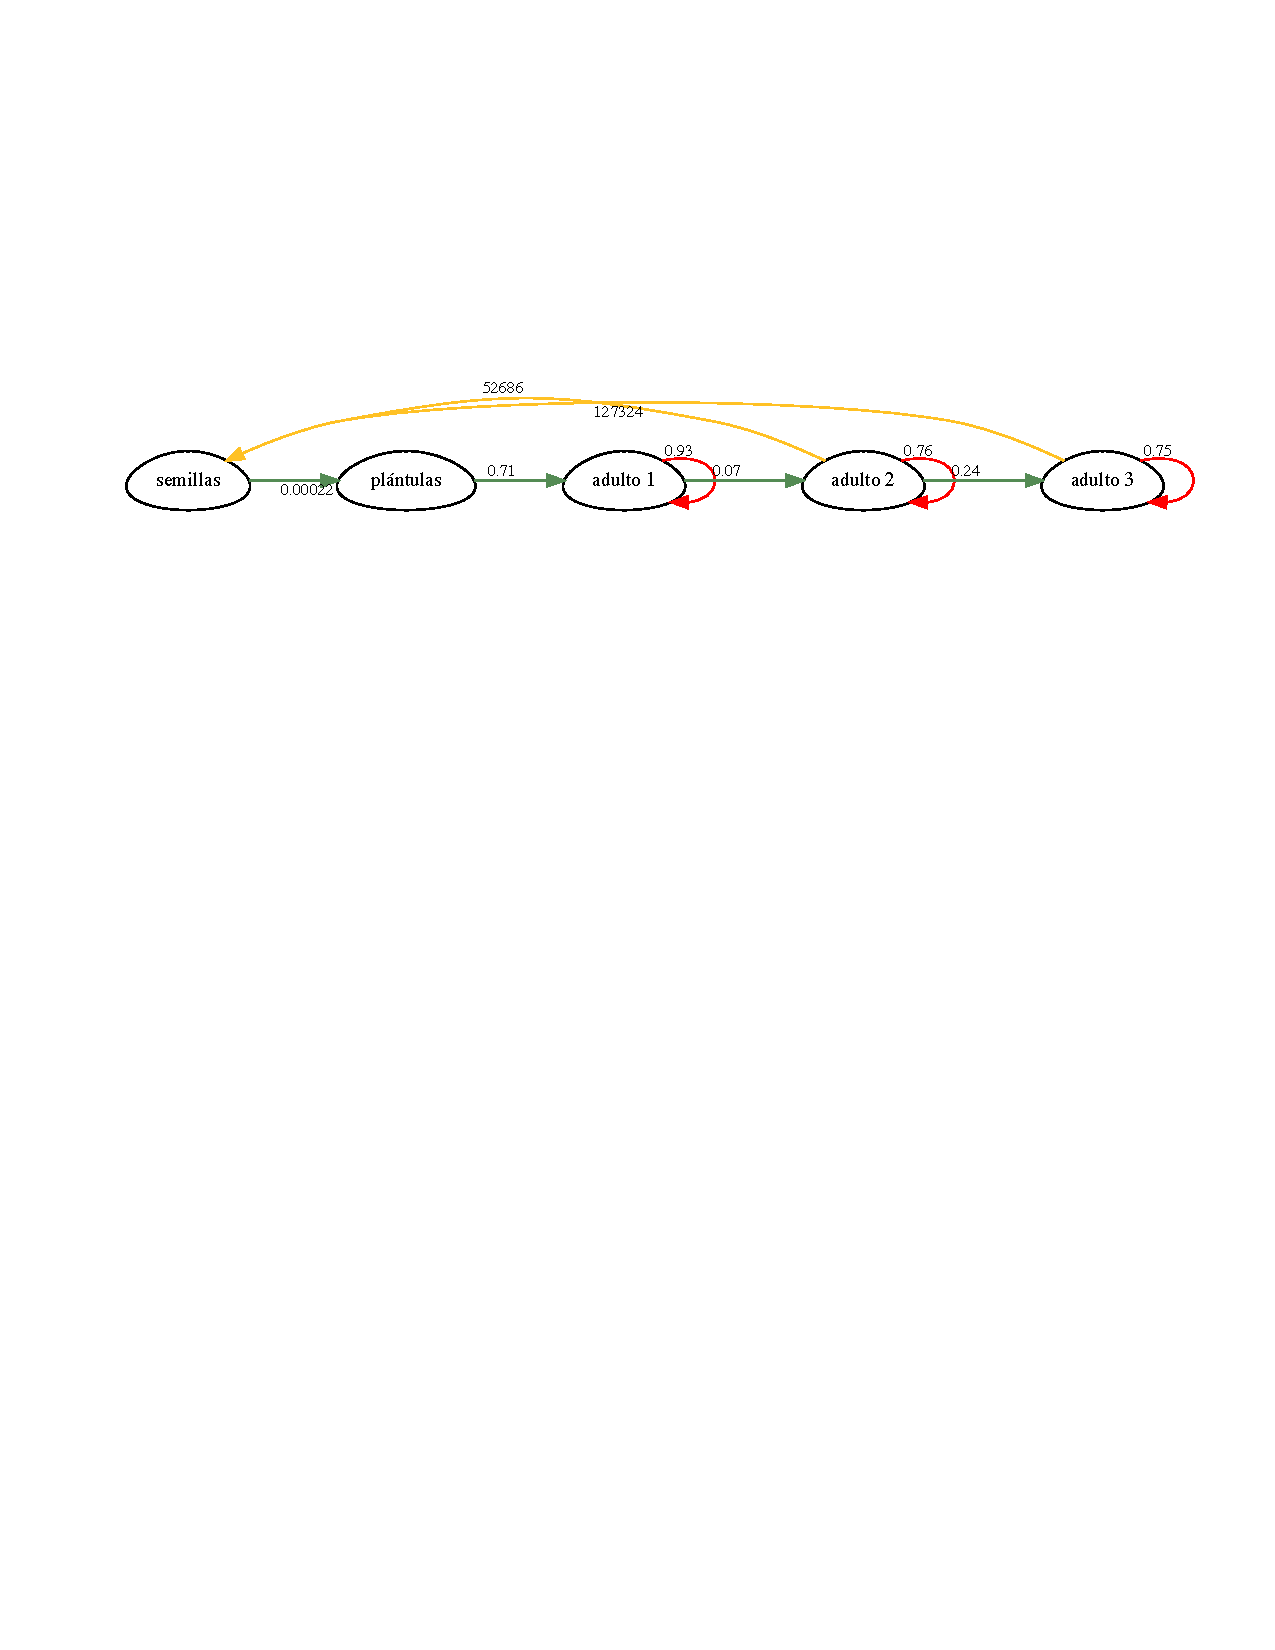
\includegraphics{103-Ciclos_de_Vida_files/figure-pdf/CV_5-1.pdf}

\subsubsection{\texorpdfstring{\emph{Telipogon
helleri}}{Telipogon helleri}}\label{telipogon-helleri}

El estudio de (Raventós et al., 2018) analizó la dinámica poblacional de
Telipogon helleri considerando tres clases de tamaño: individuos
inmaduros, adultos reproductivos pequeños y adultos reproductivos
grandes. El ciclo de vida se representó mediante tres etapas, según lo
ilustrado en la figura 1 de la publicación. El objetivo principal fue
evaluar el efecto de las perturbaciones sobre el crecimiento
poblacional, utilizando un enfoque basado en análisis de dinámica
transitoria. Los autores identificaron tres tipos de transición en la
historia de vida de la especie:

\begin{itemize}
\tightlist
\item
  Transición a una etapa subsiguiente (indicada en verde)
\item
  Permanencia en la misma etapa (flechas rojas)
\item
  Regresión en tamaño (color violeta)
\item
  Reproducción (color amarillo)
\end{itemize}

Cabe destacar que los individuos adultos grandes presentan una mayor
contribución a la producción de semillas (0.5359) en comparación con los
adultos pequeños (0.1573), lo que subraya la importancia de la
estructura de tamaños en la dinámica poblacional.

\begin{Shaded}
\begin{Highlighting}[]
\NormalTok{matA\_Th}\OtherTok{=}\FunctionTok{matrix}\NormalTok{(}\FunctionTok{c}\NormalTok{(}\FloatTok{0.1548}\NormalTok{, }\FloatTok{0.1573}\NormalTok{, }\FloatTok{0.5309}\NormalTok{,}
                 \FloatTok{0.2738}\NormalTok{, }\FloatTok{0.4425}\NormalTok{, }\FloatTok{0.1606}\NormalTok{,}
                 \FloatTok{0.0238}\NormalTok{, }\FloatTok{0.4060}\NormalTok{, }\FloatTok{0.7368}\NormalTok{), }\AttributeTok{byrow=}\ConstantTok{TRUE}\NormalTok{,}\AttributeTok{ncol=}\DecValTok{3}\NormalTok{)}

\NormalTok{matA\_Th}
\end{Highlighting}
\end{Shaded}

\begin{verbatim}
       [,1]   [,2]   [,3]
[1,] 0.1548 0.1573 0.5309
[2,] 0.2738 0.4425 0.1606
[3,] 0.0238 0.4060 0.7368
\end{verbatim}

\begin{Shaded}
\begin{Highlighting}[]
\NormalTok{etapas\_Th }\OtherTok{\textless{}{-}} \FunctionTok{c}\NormalTok{(}\StringTok{"inmaduros"}\NormalTok{, }\StringTok{"reproductivo\_pequeños"}\NormalTok{, }\StringTok{"reproductivo\_grandes"}\NormalTok{)}
\NormalTok{title }\OtherTok{\textless{}{-}} \ConstantTok{NULL}
\NormalTok{graph }\OtherTok{\textless{}{-}} \FunctionTok{expand.grid}\NormalTok{(}\AttributeTok{to =}\NormalTok{ etapas\_Th, }\AttributeTok{from =}\NormalTok{ etapas\_Th)}
\NormalTok{graph}\SpecialCharTok{$}\NormalTok{trans }\OtherTok{\textless{}{-}} \FunctionTok{round}\NormalTok{(}\FunctionTok{c}\NormalTok{(matA\_Th), }\DecValTok{3}\NormalTok{)}
\NormalTok{graph }\OtherTok{\textless{}{-}}\NormalTok{ graph[graph}\SpecialCharTok{$}\NormalTok{trans }\SpecialCharTok{\textgreater{}} \DecValTok{0}\NormalTok{, ]}
\NormalTok{nodes }\OtherTok{\textless{}{-}} \FunctionTok{paste}\NormalTok{(}\FunctionTok{paste0}\NormalTok{(}\StringTok{"\textquotesingle{}"}\NormalTok{, etapas\_Th, }\StringTok{"\textquotesingle{}"}\NormalTok{), }\AttributeTok{collapse =} \StringTok{"; "}\NormalTok{)}
\NormalTok{graph}\SpecialCharTok{$}\NormalTok{min\_len }\OtherTok{\textless{}{-}}\NormalTok{ (}\FunctionTok{as.numeric}\NormalTok{(graph}\SpecialCharTok{$}\NormalTok{to) }\SpecialCharTok{{-}} \FunctionTok{as.numeric}\NormalTok{(graph}\SpecialCharTok{$}\NormalTok{from)) }\SpecialCharTok{*} \DecValTok{3}
\NormalTok{graph}\SpecialCharTok{$}\NormalTok{col }\OtherTok{\textless{}{-}} \FunctionTok{c}\NormalTok{(}
  \StringTok{"red"}\NormalTok{, }\StringTok{"PaleGreen4"}\NormalTok{, }\StringTok{"PaleGreen4"}\NormalTok{, }
  \StringTok{"Goldenrod1"}\NormalTok{, }\StringTok{"red"}\NormalTok{, }\StringTok{"PaleGreen4"}\NormalTok{, }
  \StringTok{"Goldenrod1"}\NormalTok{, }\StringTok{"MediumOrchid4"}\NormalTok{, }\StringTok{"red"} 
\NormalTok{)}
\NormalTok{edges }\OtherTok{\textless{}{-}} \FunctionTok{paste0}\NormalTok{(}\StringTok{"\textquotesingle{}"}\NormalTok{, graph}\SpecialCharTok{$}\NormalTok{from, }\StringTok{"\textquotesingle{}"}\NormalTok{, }\StringTok{" {-}\textgreater{} "}\NormalTok{, }\StringTok{"\textquotesingle{}"}\NormalTok{, graph}\SpecialCharTok{$}\NormalTok{to, }\StringTok{"\textquotesingle{}"}\NormalTok{,}
  \StringTok{"[minlen="}\NormalTok{, graph}\SpecialCharTok{$}\NormalTok{min\_len,}
  \StringTok{",fontsize="}\NormalTok{, }\DecValTok{10}\NormalTok{,}
  \StringTok{",color="}\NormalTok{, graph}\SpecialCharTok{$}\NormalTok{col,}
  \StringTok{",xlabel="}\NormalTok{, }\FunctionTok{paste}\NormalTok{(}\StringTok{"}\SpecialCharTok{\textbackslash{}"}\StringTok{"}\NormalTok{, graph}\SpecialCharTok{$}\NormalTok{trans),}
  \StringTok{"}\SpecialCharTok{\textbackslash{}"}\StringTok{]}\SpecialCharTok{\textbackslash{}n}\StringTok{"}\NormalTok{,}
  \AttributeTok{collapse =} \StringTok{""}
\NormalTok{)}
\FunctionTok{grViz}\NormalTok{(}
  \FunctionTok{paste}\NormalTok{(}
    \StringTok{"}
\StringTok{digraph \{}
\StringTok{  \{}
\StringTok{    graph[overlap=false];}
\StringTok{    rank=same;}
\StringTok{    node [shape="}\NormalTok{, }\StringTok{"egg"}\NormalTok{, }\StringTok{", fontsize="}\NormalTok{, }\DecValTok{12}\NormalTok{, }\StringTok{"];"}\NormalTok{,}
\NormalTok{    nodes, }\StringTok{"}
\StringTok{  \}"}\NormalTok{,}
    \StringTok{"ordering=out}
\StringTok{  x [style=invis]}
\StringTok{  x {-}\textgreater{} \{"}\NormalTok{, nodes, }\StringTok{"\} [style=invis]"}\NormalTok{, edges,}
    \StringTok{"labelloc=}\SpecialCharTok{\textbackslash{}"}\StringTok{t}\SpecialCharTok{\textbackslash{}"}\StringTok{;}
\StringTok{  label=}\SpecialCharTok{\textbackslash{}"}\StringTok{"}\NormalTok{, title, }\StringTok{"}\SpecialCharTok{\textbackslash{}"}
\StringTok{\}"}
\NormalTok{  )}
\NormalTok{) }
\end{Highlighting}
\end{Shaded}

\begin{verbatim}
file:////private/var/folders/3k/1ft37x9130vdbz21tw1497x40000gn/T/RtmpTIXuwN/file1061a23c6b3f8/widget1061a4a517121.html screenshot completed
\end{verbatim}

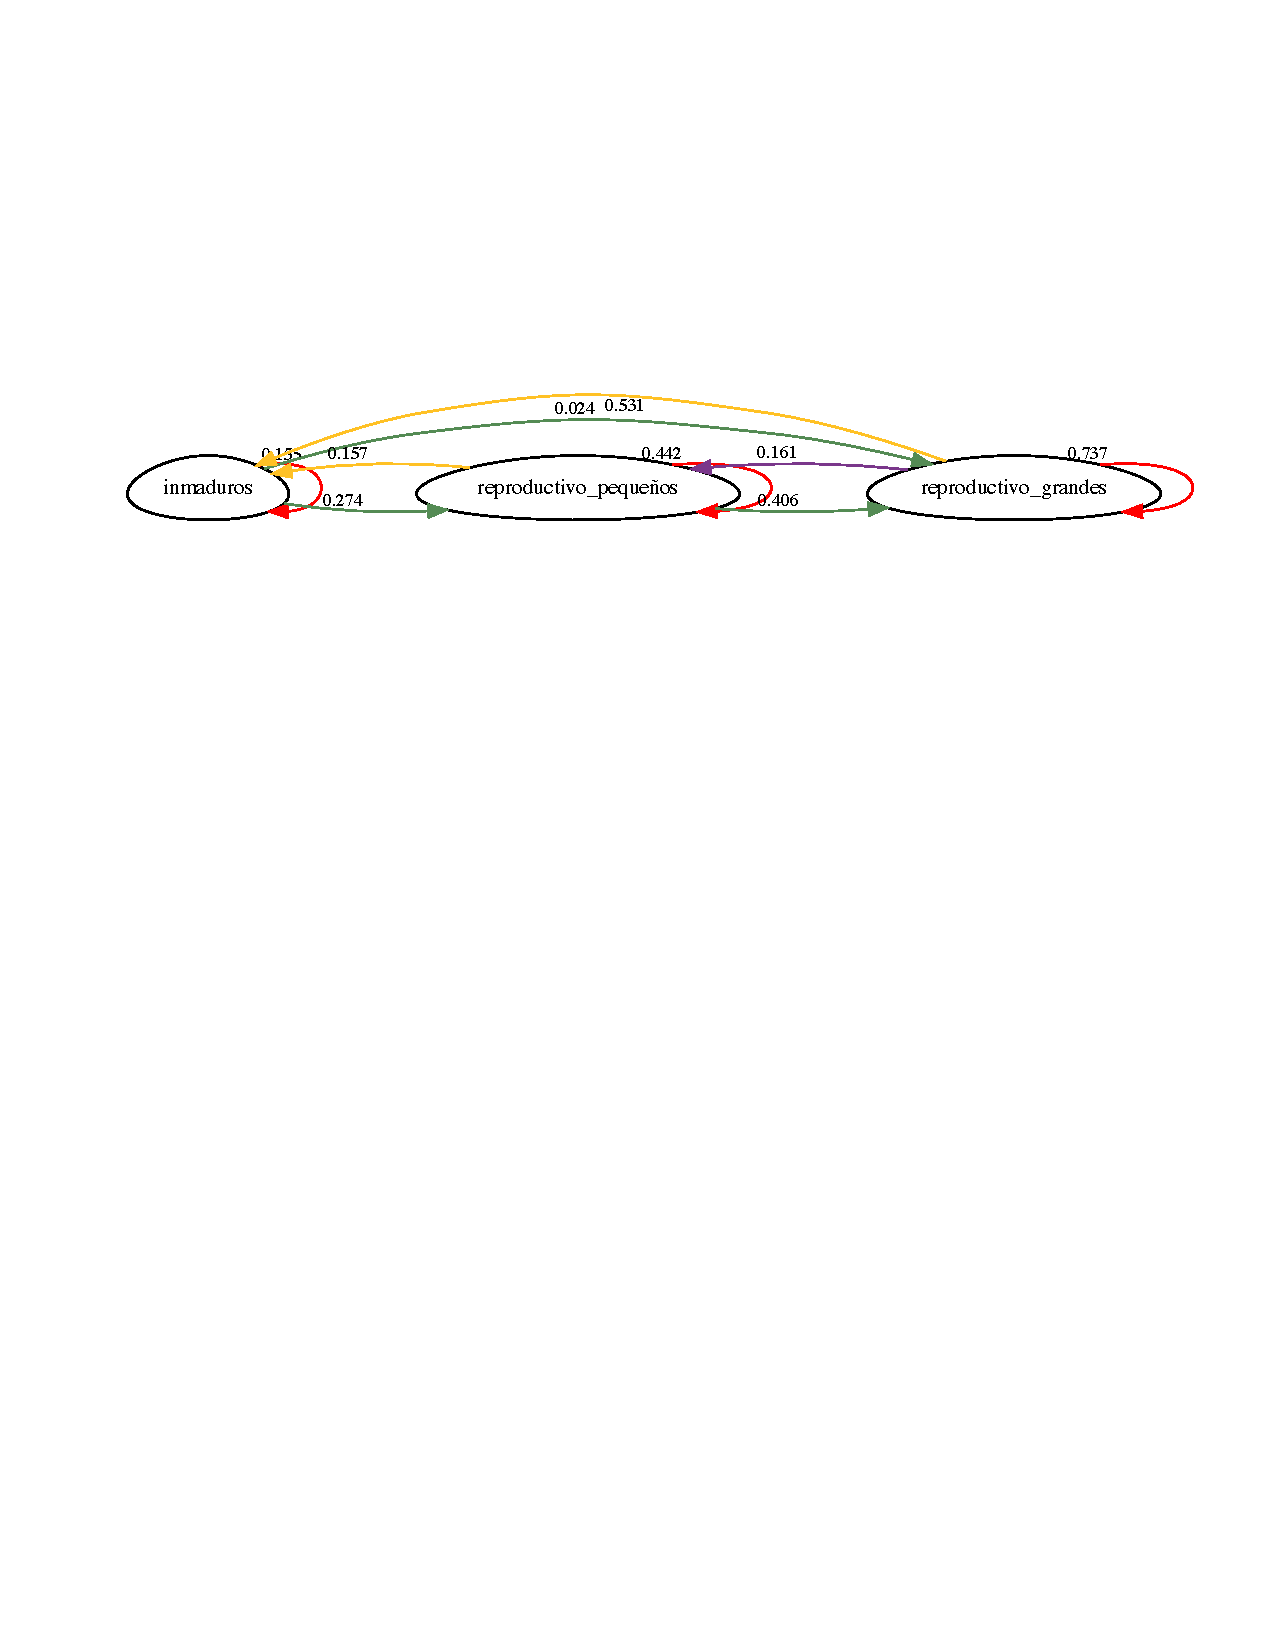
\includegraphics{103-Ciclos_de_Vida_files/figure-pdf/CV_6Telipogon_helleri-1.pdf}

\subsection{Especies Terrestres}\label{especies-terrestres}

\subsubsection{\texorpdfstring{\emph{Prasophyllum
correctum}}{Prasophyllum correctum}}\label{prasophyllum-correctum}

En el trabajo de Coates y colaboradores con \emph{Prasophyllum
correctum} se recolectaron datos de la etapa de plántula, juvenil,
adulto y latencia de los individuos (Coates, Lunt \& Tremblay, 2006). La
historia de vida de la especie está representada por 4 etapas. Los datos
provienen de la figura 4 de la publicación de (Coates, Lunt \& Tremblay,
2006), donde hay un periodo de 3 o más años entre los periodos de
régimen de fuegos. Una de la etapas distintivas de esta especie es la
latencia vegetativa, lo que significa que las plantas no emergen cada
año sus tubérculos (estructura de perennación) se mantienen vivos debajo
del suelo. Muchas especies de orquídeas terrestres tienen latencia en
las etapas de plántulas, juvenil y adultos.

En \emph{P. correctum}, al igual que en otras especies terrestres, es
difícil estimar su muerte debido a la presencia de latencia vegetativa.
Esto típicamente es un problema de muestreo y no de la biología de la
especie, ya que es muy difícil estimar la muerte de los individuos. La
ausencia de una planta marcada no significa que este muerte, sino que
potencialmente está en su fase latente. Poder diferencia un estado de
otro, también es difícil, ya que no es ético modificar el hábitat para
determinar si la planta esta viva o muerta, más aún si condieramos que
muchas de las especies terrestres están en peligro de extinción. Una
manera de dar solición a esta situación es hacer unos análisis para
determinar cuál es la probabilidad de que esté vivo un individuo con
latencia vegetativa de múltiples años. En este caso, se hace unos
análisis usando análisis bayesiano (Tremblay et al., 2009) para
determinar cual es la probabilidad que un individuo con latencia de
múltiples

El tránsito a la fase de latencia vegetativa se indica en azul, en verde
el crecimiento, en amarillo la reproducción y en rojo la permanencia en
una misma etapa, incluyendo latente a latente.

\begin{Shaded}
\begin{Highlighting}[]
\NormalTok{matA\_lat }\OtherTok{\textless{}{-}} \FunctionTok{rbind}\NormalTok{(}
  \FunctionTok{c}\NormalTok{(}\FloatTok{0.0}\NormalTok{,     }\FloatTok{0.0}\NormalTok{,  }\FloatTok{0.0125}\NormalTok{,  }\FloatTok{0.0000}\NormalTok{),}
  \FunctionTok{c}\NormalTok{(}\FloatTok{0.0}\NormalTok{,  }\FloatTok{0.2874}\NormalTok{,  }\FloatTok{0.3750}\NormalTok{,  }\FloatTok{0.1364}\NormalTok{),}
  \FunctionTok{c}\NormalTok{(}\FloatTok{0.0}\NormalTok{,  }\FloatTok{0.0230}\NormalTok{,  }\FloatTok{0.1500}\NormalTok{,  }\FloatTok{0.0303}\NormalTok{),}
  \FunctionTok{c}\NormalTok{(}\FloatTok{1.0}\NormalTok{,  }\FloatTok{0.6897}\NormalTok{,   }\FloatTok{0.4750}\NormalTok{,  }\FloatTok{0.7475}\NormalTok{) }
\NormalTok{)}


\NormalTok{etapas\_lat }\OtherTok{\textless{}{-}} \FunctionTok{c}\NormalTok{(}\StringTok{"plántulas"}\NormalTok{, }\StringTok{"adultos vegetativos"}\NormalTok{, }\StringTok{"adultos reproductivos"}\NormalTok{, }\StringTok{"latencia"}\NormalTok{)}
\NormalTok{title }\OtherTok{\textless{}{-}} \ConstantTok{NULL}
\NormalTok{graph }\OtherTok{\textless{}{-}} \FunctionTok{expand.grid}\NormalTok{(}\AttributeTok{to =}\NormalTok{ etapas\_lat, }\AttributeTok{from =}\NormalTok{ etapas\_lat)}
\NormalTok{graph}\SpecialCharTok{$}\NormalTok{trans }\OtherTok{\textless{}{-}} \FunctionTok{round}\NormalTok{(}\FunctionTok{c}\NormalTok{(matA\_lat), }\DecValTok{4}\NormalTok{)}
\NormalTok{graph }\OtherTok{\textless{}{-}}\NormalTok{ graph[graph}\SpecialCharTok{$}\NormalTok{trans }\SpecialCharTok{\textgreater{}} \DecValTok{0}\NormalTok{, ]}
\NormalTok{nodes }\OtherTok{\textless{}{-}} \FunctionTok{paste}\NormalTok{(}\FunctionTok{paste0}\NormalTok{(}\StringTok{"\textquotesingle{}"}\NormalTok{, etapas\_lat, }\StringTok{"\textquotesingle{}"}\NormalTok{), }\AttributeTok{collapse =} \StringTok{"; "}\NormalTok{)}
\NormalTok{graph}\SpecialCharTok{$}\NormalTok{min\_len }\OtherTok{\textless{}{-}}\NormalTok{ (}\FunctionTok{as.numeric}\NormalTok{(graph}\SpecialCharTok{$}\NormalTok{to) }\SpecialCharTok{{-}} \FunctionTok{as.numeric}\NormalTok{(graph}\SpecialCharTok{$}\NormalTok{from)) }\SpecialCharTok{*} \DecValTok{2}
\NormalTok{graph}\SpecialCharTok{$}\NormalTok{col }\OtherTok{\textless{}{-}} \FunctionTok{c}\NormalTok{(}
  \StringTok{"black"}\NormalTok{, }
  \StringTok{"red"}\NormalTok{, }\StringTok{"palegreen4"}\NormalTok{, }\StringTok{"black"}\NormalTok{,}
  \StringTok{"goldenrod1"}\NormalTok{, }\StringTok{"blue"}\NormalTok{, }\StringTok{"red"}\NormalTok{, }\StringTok{"black"}\NormalTok{,}
  \StringTok{"blue"}\NormalTok{, }\StringTok{"blue"}\NormalTok{, }\StringTok{"red"}
\NormalTok{)}
\NormalTok{edges }\OtherTok{\textless{}{-}} \FunctionTok{paste0}\NormalTok{(}\StringTok{"\textquotesingle{}"}\NormalTok{, graph}\SpecialCharTok{$}\NormalTok{from, }\StringTok{"\textquotesingle{}"}\NormalTok{, }\StringTok{" {-}\textgreater{} "}\NormalTok{, }\StringTok{"\textquotesingle{}"}\NormalTok{, graph}\SpecialCharTok{$}\NormalTok{to, }\StringTok{"\textquotesingle{}"}\NormalTok{,}
  \StringTok{"[minlen="}\NormalTok{, graph}\SpecialCharTok{$}\NormalTok{min\_len,}
  \StringTok{",fontsize="}\NormalTok{, }\DecValTok{10}\NormalTok{,}
  \StringTok{",color="}\NormalTok{, graph}\SpecialCharTok{$}\NormalTok{col,}
  \StringTok{",xlabel="}\NormalTok{, }\FunctionTok{paste}\NormalTok{(}\StringTok{"}\SpecialCharTok{\textbackslash{}"}\StringTok{"}\NormalTok{, graph}\SpecialCharTok{$}\NormalTok{trans),}
  \StringTok{"}\SpecialCharTok{\textbackslash{}"}\StringTok{]}\SpecialCharTok{\textbackslash{}n}\StringTok{"}\NormalTok{,}
  \AttributeTok{collapse =} \StringTok{""}
\NormalTok{)}
\FunctionTok{grViz}\NormalTok{(}
  \FunctionTok{paste}\NormalTok{(}
    \StringTok{"}
\StringTok{digraph \{}
\StringTok{  \{}
\StringTok{    graph[overlap=false];}
\StringTok{    rank=same;}
\StringTok{    node [shape="}\NormalTok{, }\StringTok{"egg"}\NormalTok{, }\StringTok{", fontsize="}\NormalTok{, }\DecValTok{12}\NormalTok{, }\StringTok{"];"}\NormalTok{,}
\NormalTok{    nodes, }\StringTok{"}
\StringTok{  \}"}\NormalTok{,}
    \StringTok{"ordering=out}
\StringTok{  x [style=invis]}
\StringTok{  x {-}\textgreater{} \{"}\NormalTok{, nodes, }\StringTok{"\} [style=invis]"}\NormalTok{, edges,}
    \StringTok{"labelloc=}\SpecialCharTok{\textbackslash{}"}\StringTok{t}\SpecialCharTok{\textbackslash{}"}\StringTok{;}
\StringTok{  label=}\SpecialCharTok{\textbackslash{}"}\StringTok{"}\NormalTok{, title, }\StringTok{"}\SpecialCharTok{\textbackslash{}"}
\StringTok{\}"}
\NormalTok{  )}
\NormalTok{) }
\end{Highlighting}
\end{Shaded}

\begin{verbatim}
file:////private/var/folders/3k/1ft37x9130vdbz21tw1497x40000gn/T/RtmpTIXuwN/file1061a1b1520e7/widget1061a8232b95.html screenshot completed
\end{verbatim}

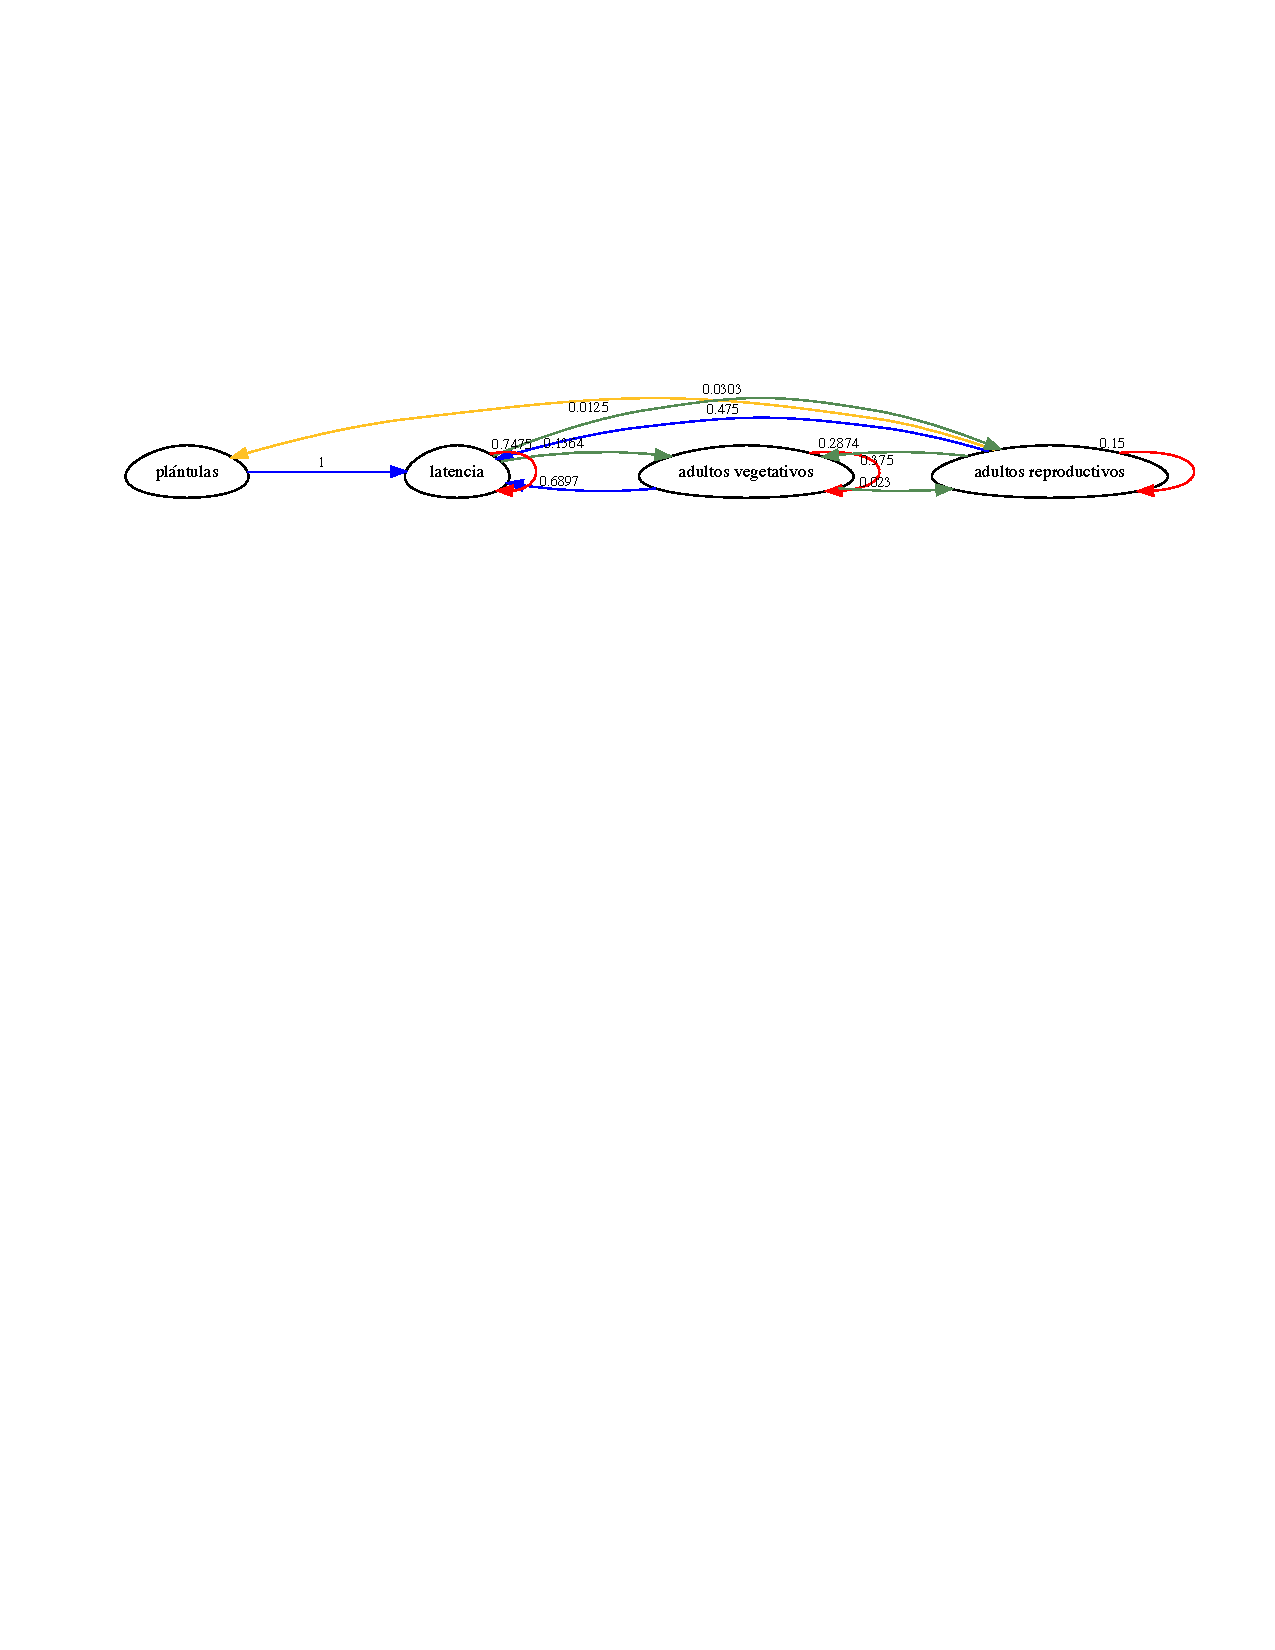
\includegraphics{103-Ciclos_de_Vida_files/figure-pdf/CV7Prasophyllum_correctum-1.pdf}

\subsubsection{\texorpdfstring{\emph{Ophrys
sphegodes}}{Ophrys sphegodes}}\label{ophrys-sphegodes}

En el trabajo de Waite y Hutchings 1991 con \emph{Ophrys sphegodes}, se
recolectaron datos de la etapa vegetativa, plantas en flor y latencia de
un año y dos años, por consecuencia la historia de vida está
representada por 4 etapas. Los datos provienen de la figura 1 y la tabla
3b (periodo de herbivoría por oveja) de la publicación de (periodo de
herbivoría por oveja) de la publicación de (Waite \& Hutchings, 1991).
). En este caso, se hace análisis para determinar cuál es la
probabilidad que un individuo con latencia vegetativa múltiple (uno o
dos años) este vivo al comparar poblaciones que están sujetas a la
herbivoría por ovejas o ganado.

Dado que el análisis se enfoca en la sobrevivencia, en el estudio no se
incluye la reproducción (no hay línea amarilla). Las etapas que pasen a
latente el siguiente año se señalan en azul, las que se quedan en la
misma etapa están en rojo, mientras que en verde el tránsito a una etapa
no latente.

\begin{Shaded}
\begin{Highlighting}[]
\NormalTok{G1}\OtherTok{=}\FunctionTok{matrix}\NormalTok{(}\FunctionTok{c}\NormalTok{(}\FloatTok{0.0080}\NormalTok{, }\FloatTok{0.0184}\NormalTok{,   }\FloatTok{0.0149}\NormalTok{, }\FloatTok{0.0148}\NormalTok{,}
            \FloatTok{0.0180}\NormalTok{,  }\FloatTok{0.4249}\NormalTok{,  }\FloatTok{0.1214}\NormalTok{, }\FloatTok{0.1214}\NormalTok{,}
            \FloatTok{0.1853}\NormalTok{,  }\FloatTok{0.2770}\NormalTok{,  }\DecValTok{0}\NormalTok{,      }\DecValTok{0}\NormalTok{,}
            \DecValTok{0}\NormalTok{,       }\DecValTok{0}\NormalTok{,       }\FloatTok{0.3050}\NormalTok{, }\DecValTok{0}\NormalTok{), }\AttributeTok{byrow=}\ConstantTok{TRUE}\NormalTok{,}\AttributeTok{ncol=}\DecValTok{4}\NormalTok{)}


\NormalTok{etapas\_Op }\OtherTok{\textless{}{-}} \FunctionTok{c}\NormalTok{(}\StringTok{"Vegetativa"}\NormalTok{, }\StringTok{"Ind. con Flores"}\NormalTok{, }\StringTok{"Latencia año 1"}\NormalTok{, }\StringTok{"Latencia año 2"}\NormalTok{)}
\NormalTok{title }\OtherTok{\textless{}{-}} \ConstantTok{NULL}
\NormalTok{graph }\OtherTok{\textless{}{-}} \FunctionTok{expand.grid}\NormalTok{(}\AttributeTok{to =}\NormalTok{ etapas\_Op, }\AttributeTok{from =}\NormalTok{ etapas\_Op)}
\NormalTok{graph}\SpecialCharTok{$}\NormalTok{trans }\OtherTok{\textless{}{-}} \FunctionTok{round}\NormalTok{(}\FunctionTok{c}\NormalTok{(G1), }\DecValTok{4}\NormalTok{)}
\NormalTok{graph }\OtherTok{\textless{}{-}}\NormalTok{ graph[graph}\SpecialCharTok{$}\NormalTok{trans }\SpecialCharTok{\textgreater{}} \DecValTok{0}\NormalTok{, ]}
\NormalTok{nodes }\OtherTok{\textless{}{-}} \FunctionTok{paste}\NormalTok{(}\FunctionTok{paste0}\NormalTok{(}\StringTok{"\textquotesingle{}"}\NormalTok{, etapas\_Op, }\StringTok{"\textquotesingle{}"}\NormalTok{), }\AttributeTok{collapse =} \StringTok{"; "}\NormalTok{)}
\NormalTok{graph}\SpecialCharTok{$}\NormalTok{min\_len }\OtherTok{\textless{}{-}}\NormalTok{ (}\FunctionTok{as.numeric}\NormalTok{(graph}\SpecialCharTok{$}\NormalTok{to) }\SpecialCharTok{{-}} \FunctionTok{as.numeric}\NormalTok{(graph}\SpecialCharTok{$}\NormalTok{from)) }\SpecialCharTok{*} \DecValTok{2}
\NormalTok{graph}\SpecialCharTok{$}\NormalTok{col }\OtherTok{\textless{}{-}} \FunctionTok{c}\NormalTok{(}
  \StringTok{"red"}\NormalTok{, }\StringTok{"PaleGreen4"}\NormalTok{, }\StringTok{"blue"}\NormalTok{,}
  \StringTok{"PaleGreen4"}\NormalTok{, }\StringTok{"red"}\NormalTok{, }\StringTok{"blue"}\NormalTok{,}
  \StringTok{"PaleGreen4"}\NormalTok{, }\StringTok{"PaleGreen4"}\NormalTok{,  }\StringTok{"blue"}\NormalTok{,}
  \StringTok{"PaleGreen4"}\NormalTok{, }\StringTok{"PaleGreen4"}
\NormalTok{)}
\NormalTok{edges }\OtherTok{\textless{}{-}} \FunctionTok{paste0}\NormalTok{(}\StringTok{"\textquotesingle{}"}\NormalTok{, graph}\SpecialCharTok{$}\NormalTok{from, }\StringTok{"\textquotesingle{}"}\NormalTok{, }\StringTok{" {-}\textgreater{} "}\NormalTok{, }\StringTok{"\textquotesingle{}"}\NormalTok{, graph}\SpecialCharTok{$}\NormalTok{to, }\StringTok{"\textquotesingle{}"}\NormalTok{,}
  \StringTok{"[minlen="}\NormalTok{, graph}\SpecialCharTok{$}\NormalTok{min\_len,}
  \StringTok{",fontsize="}\NormalTok{, }\DecValTok{10}\NormalTok{,}
  \StringTok{",color="}\NormalTok{, graph}\SpecialCharTok{$}\NormalTok{col,}
  \StringTok{",xlabel="}\NormalTok{, }\FunctionTok{paste}\NormalTok{(}\StringTok{"}\SpecialCharTok{\textbackslash{}"}\StringTok{"}\NormalTok{, graph}\SpecialCharTok{$}\NormalTok{trans),}
  \StringTok{"}\SpecialCharTok{\textbackslash{}"}\StringTok{]}\SpecialCharTok{\textbackslash{}n}\StringTok{"}\NormalTok{,}
  \AttributeTok{collapse =} \StringTok{""}
\NormalTok{)}
\FunctionTok{grViz}\NormalTok{(}
  \FunctionTok{paste}\NormalTok{(}
    \StringTok{"}
\StringTok{digraph \{}
\StringTok{  \{}
\StringTok{    graph[overlap=false];}
\StringTok{    rank=same;}
\StringTok{    node [shape="}\NormalTok{, }\StringTok{"egg"}\NormalTok{, }\StringTok{", fontsize="}\NormalTok{, }\DecValTok{12}\NormalTok{, }\StringTok{"];"}\NormalTok{,}
\NormalTok{    nodes, }\StringTok{"}
\StringTok{  \}"}\NormalTok{,}
    \StringTok{"ordering=out}
\StringTok{  x [style=invis]}
\StringTok{  x {-}\textgreater{} \{"}\NormalTok{, nodes, }\StringTok{"\} [style=invis]"}\NormalTok{, edges,}
    \StringTok{"labelloc=}\SpecialCharTok{\textbackslash{}"}\StringTok{t}\SpecialCharTok{\textbackslash{}"}\StringTok{;}
\StringTok{  label=}\SpecialCharTok{\textbackslash{}"}\StringTok{"}\NormalTok{, title, }\StringTok{"}\SpecialCharTok{\textbackslash{}"}
\StringTok{\}"}
\NormalTok{  )}
\NormalTok{) }
\end{Highlighting}
\end{Shaded}

\begin{verbatim}
file:////private/var/folders/3k/1ft37x9130vdbz21tw1497x40000gn/T/RtmpTIXuwN/file1061a11e494b3/widget1061a35de7cf2.html screenshot completed
\end{verbatim}

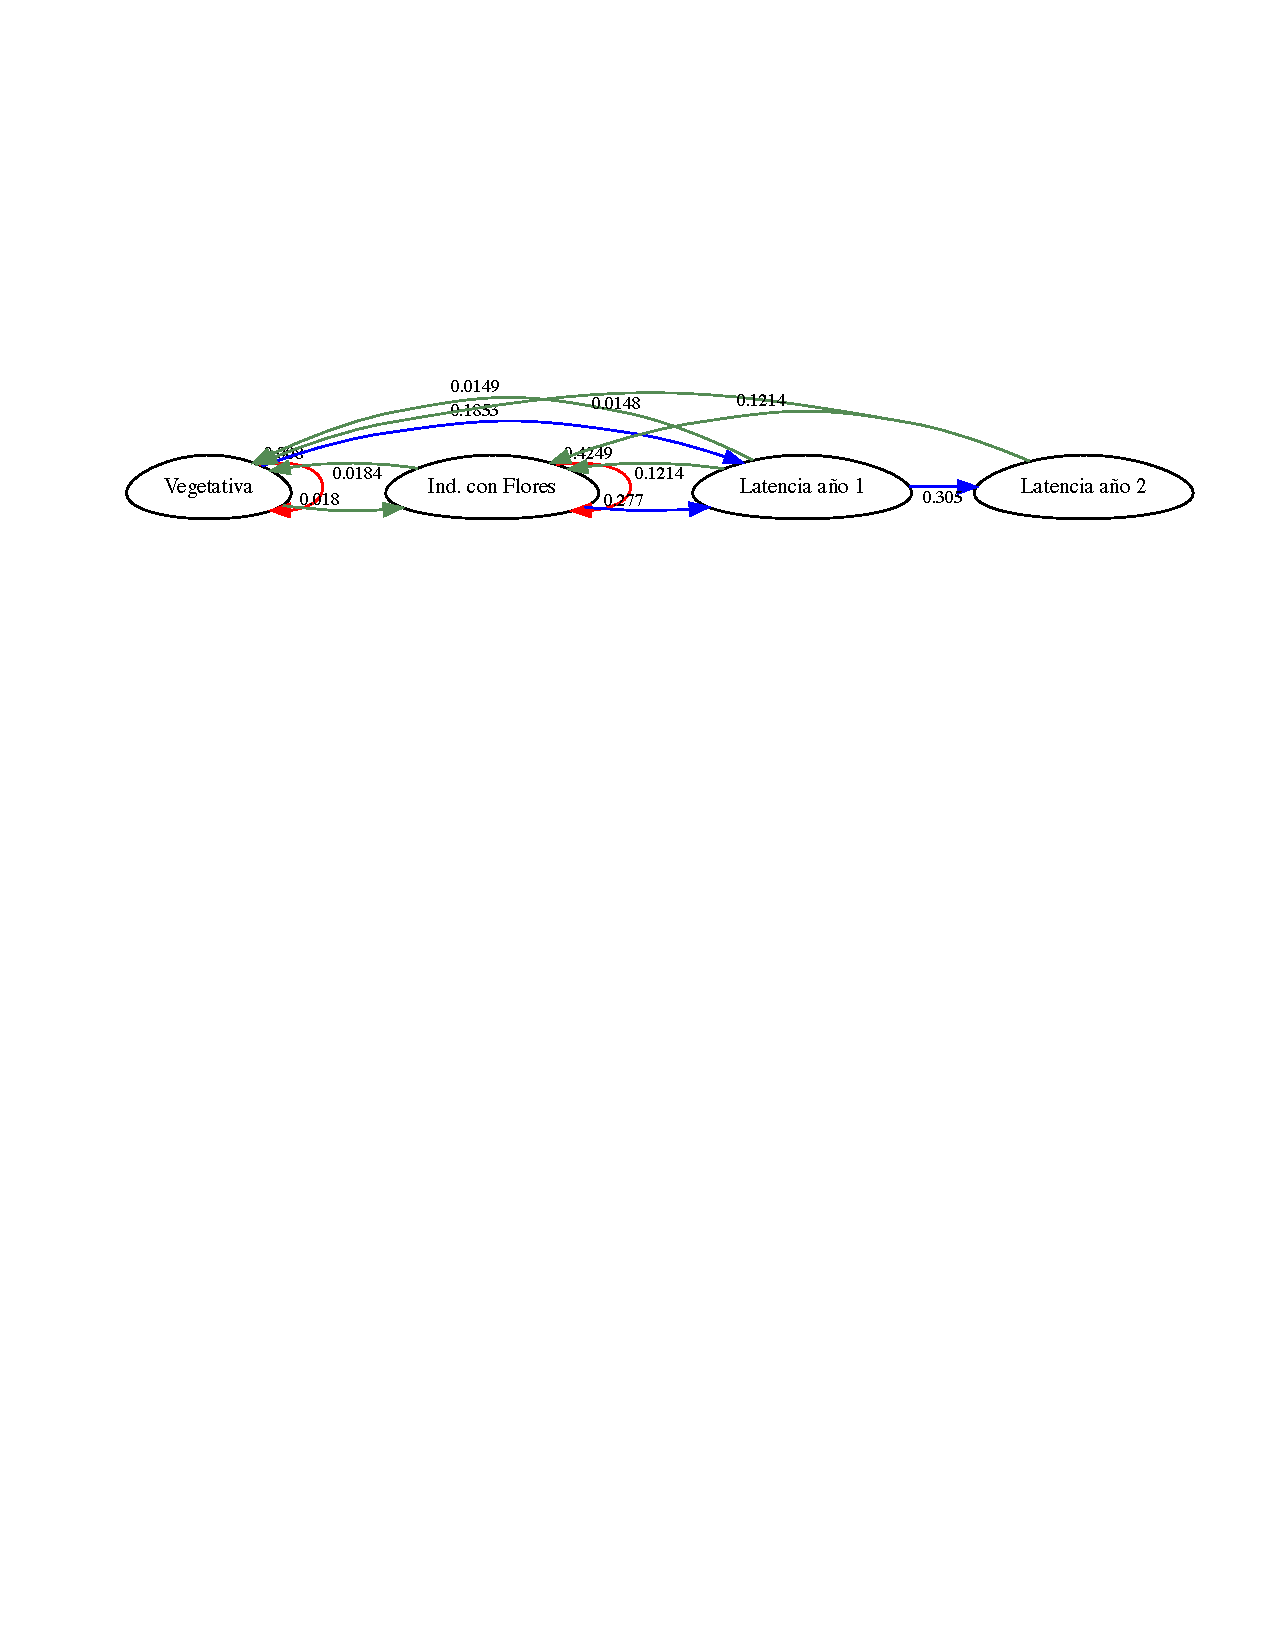
\includegraphics{103-Ciclos_de_Vida_files/figure-pdf/CV8_Ophrys-1.pdf}

\subsubsection{\texorpdfstring{\emph{Cypripedium parviflorum},
\emph{Epipactus atrorubens} y \emph{Orchis
purpurea}}{Cypripedium parviflorum, Epipactus atrorubens y Orchis purpurea}}\label{cypripedium-parviflorum-epipactus-atrorubens-y-orchis-purpurea}

\begin{figure}[H]

{\centering 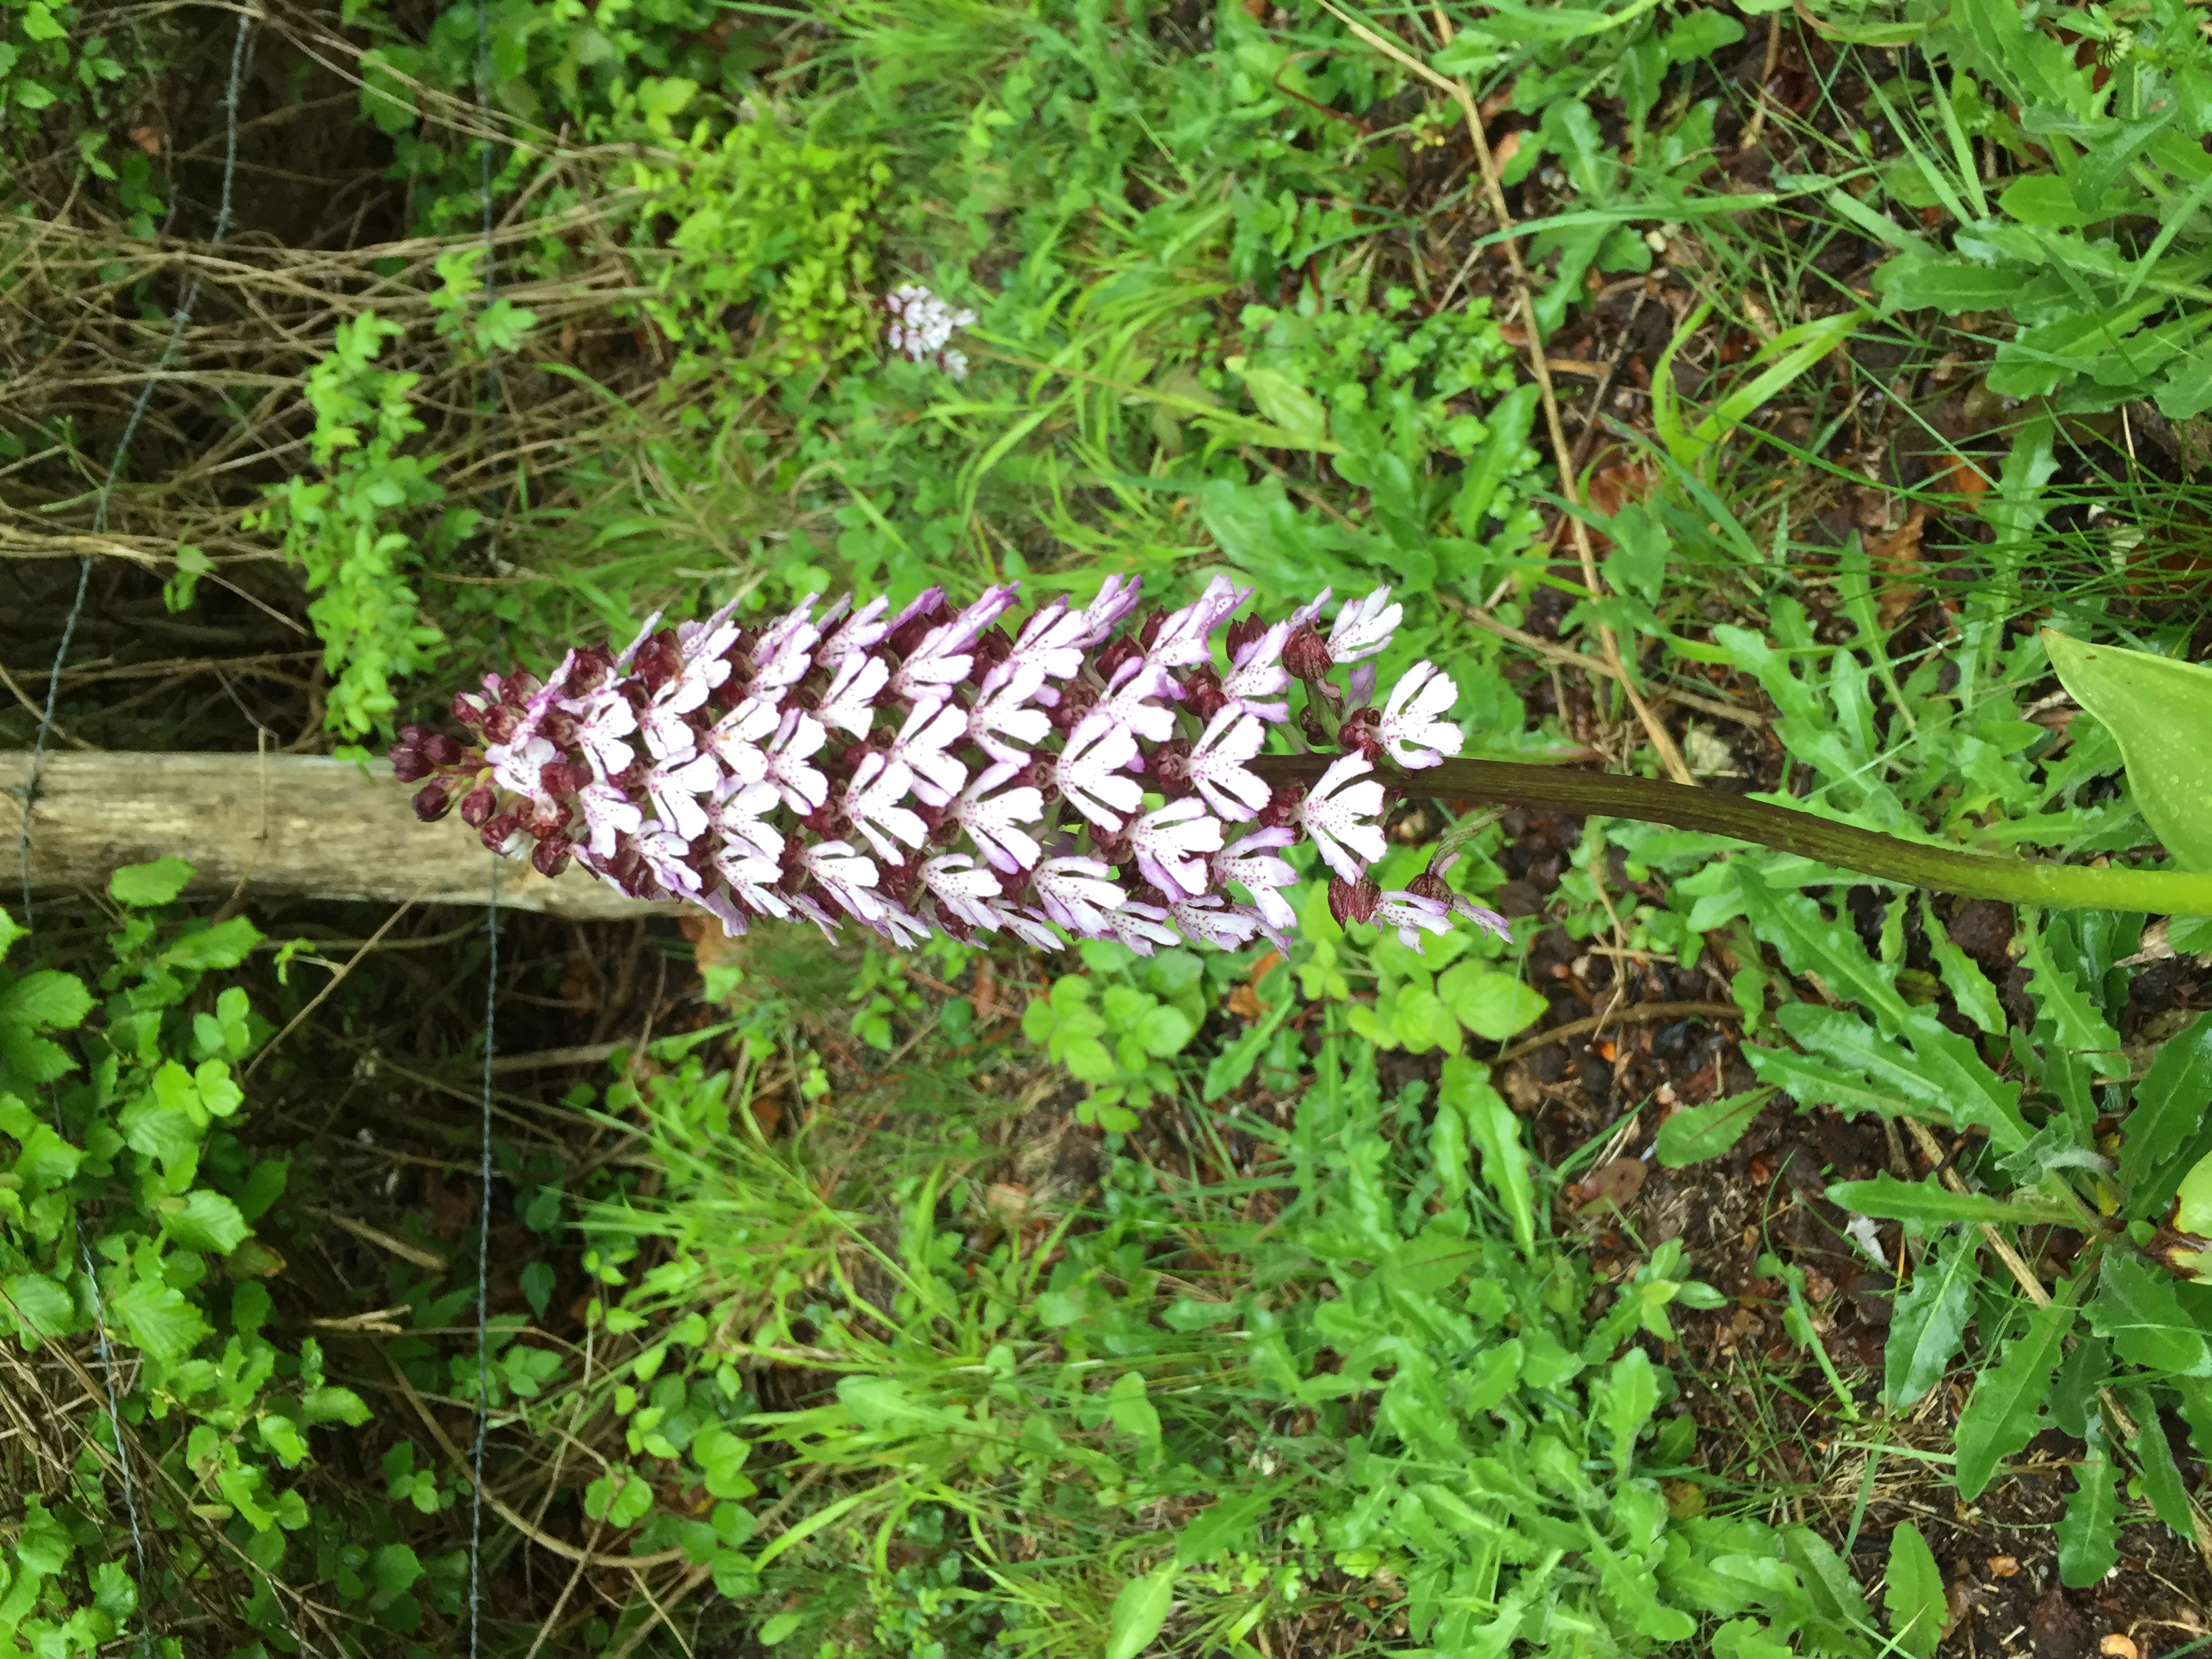
\includegraphics{Species/Orchis purpurea 1 Hans Jacquemyn.jpg}

}

\caption{\emph{Orchis purpurea}. Foto: Hans Jacquemyn}

\end{figure}%

La dimensiones de la matriz y la cantidad de etapas o años incluidos en
un análisis depende de múltiples factores. Cuando se trabaja con datos
de campo, el acceso a individuos de cada etapa del ciclo de vida es, sin
duda, un factor determinante. En la revisión de la publicaciones sobre
orquídeas se encuentran análisis matriciales que varían entre 3 y 29
etapas de desarrollo, en promedio 5.6 etapas (desv. estandard de 3.2).
El trabajo con mayor número de etapas es el de (Shefferson, Warren \&
Pulliam, 2014), que utilizó 29 en \emph{Cypripedium parviflorum} var.
\emph{parviflorum}.

El costo de pasar a una fase latente después de diferentes etapas se
evaluó en \emph{Epipactus atrorubens}. En este análisis se definieron 11
estados, considerando la posibilidad de entrar en latencia vegetativa
desde todas estas fases emergentes (Jäkäläniemi et al., 2011). En
\emph{Orchis purpurea}, los autores modelaron el diagrama del ciclo de
vida, definiendo 6 etapas de desarrollo: protocormos, turberculos,
plántulas, juveniles (más de un año y menos de 3 hojas), plantas sin
flores (más de 3 hojas) y plantas con flores, a continuación se presenta
la matriz correspondiente tomada de (Jacquemyn, Brys \& Jongejans,
2010). La transiciones a una etapa subsiguiente se señalan en verde, en
violeta las transiciones a una etapa más pequeña y la reproducción en
amarillo. En este ciclo de vida las etapas de protocormos, tuberculos,
plántulas son de un año cada una. Si estos individuos no crecen a la
próxima etapa se supone que mueren.

\begin{figure}[H]

{\centering 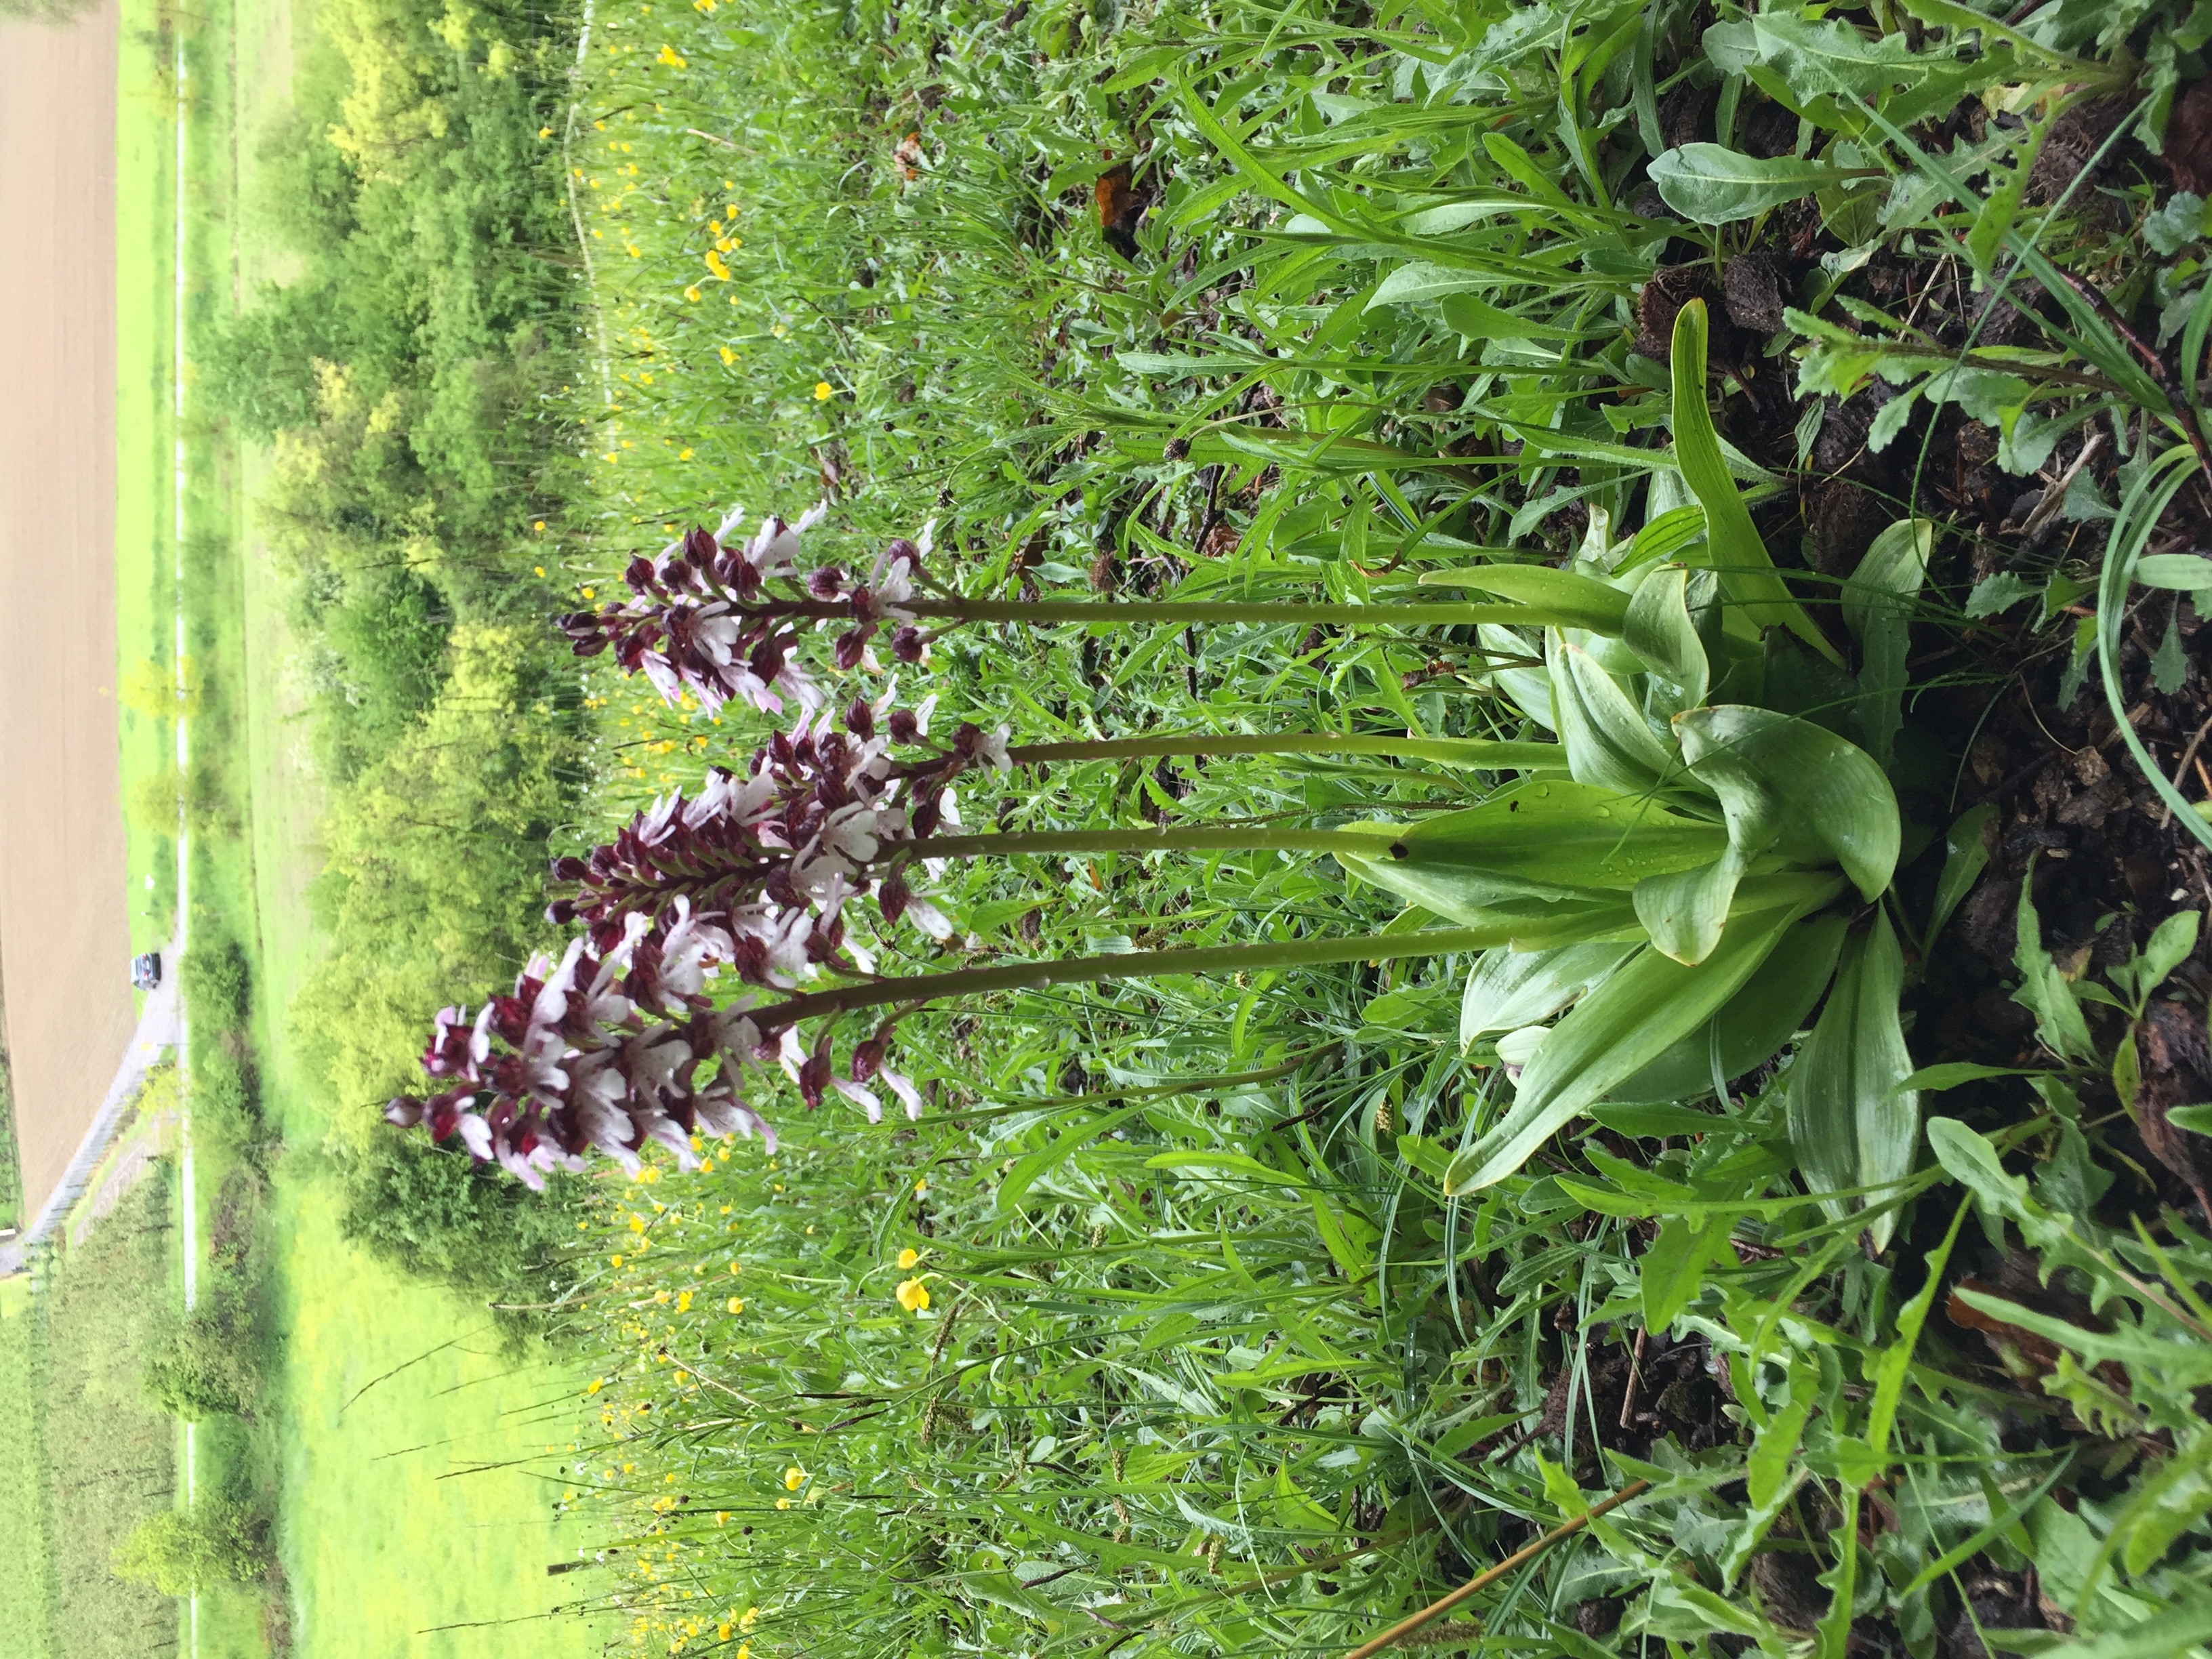
\includegraphics{Species/Orchis_purpurea_2_Hans_Jacquemyn.jpg}

}

\caption{\emph{Orchis purpurea}. Foto: Hans Jacquemyn}

\end{figure}%

Aquí se visualiza la matriz de \emph{Orchis purpurea} de la publicación
de. La transiciones a una etapa subsiguiente son en verde, las
transiciones a una etapa más pequeña son en violeta y la reproducción en
amarillo. En este ciclo de vida las etapas de protocormos, tubérculos,
plántulas son de un año cada una. Si estos individuos no crecen a la
próxima etapa se asume que fallecieron.

\[\\[1in]\]

\begin{Shaded}
\begin{Highlighting}[]
\NormalTok{matA\_Os}\OtherTok{=}\FunctionTok{matrix}\NormalTok{(}\FunctionTok{c}\NormalTok{(}
\FloatTok{0.000}\NormalTok{, }\FloatTok{0.000}\NormalTok{, }\DecValTok{0}\NormalTok{, }\FloatTok{0.00}\NormalTok{, }\FloatTok{0.000}\NormalTok{, }\FloatTok{84.88725}\NormalTok{,}
\FloatTok{0.012}\NormalTok{, }\FloatTok{0.000}\NormalTok{, }\DecValTok{0}\NormalTok{, }\FloatTok{0.00}\NormalTok{, }\FloatTok{0.000}\NormalTok{,  }\FloatTok{0.00000}\NormalTok{,}
\FloatTok{0.000}\NormalTok{, }\FloatTok{0.041}\NormalTok{, }\DecValTok{0}\NormalTok{, }\FloatTok{0.00}\NormalTok{, }\FloatTok{0.000}\NormalTok{,  }\FloatTok{0.00000}\NormalTok{,}
\FloatTok{0.000}\NormalTok{, }\FloatTok{0.000}\NormalTok{, }\DecValTok{1}\NormalTok{, }\FloatTok{0.75}\NormalTok{, }\FloatTok{0.000}\NormalTok{,  }\FloatTok{0.00000}\NormalTok{,}
\FloatTok{0.000}\NormalTok{, }\FloatTok{0.000}\NormalTok{, }\DecValTok{0}\NormalTok{, }\FloatTok{0.25}\NormalTok{, }\FloatTok{0.615}\NormalTok{,  }\FloatTok{0.62500}\NormalTok{,}
\FloatTok{0.000}\NormalTok{, }\FloatTok{0.000}\NormalTok{, }\DecValTok{0}\NormalTok{, }\FloatTok{0.00}\NormalTok{, }\FloatTok{0.385}\NormalTok{,  }\FloatTok{0.37500}\NormalTok{), }\AttributeTok{byrow=}\ConstantTok{TRUE}\NormalTok{,}\AttributeTok{ncol=}\DecValTok{6}\NormalTok{)}

\NormalTok{matA\_Os  }
\end{Highlighting}
\end{Shaded}

\begin{verbatim}
      [,1]  [,2] [,3] [,4]  [,5]     [,6]
[1,] 0.000 0.000    0 0.00 0.000 84.88725
[2,] 0.012 0.000    0 0.00 0.000  0.00000
[3,] 0.000 0.041    0 0.00 0.000  0.00000
[4,] 0.000 0.000    1 0.75 0.000  0.00000
[5,] 0.000 0.000    0 0.25 0.615  0.62500
[6,] 0.000 0.000    0 0.00 0.385  0.37500
\end{verbatim}

\begin{center}\rule{0.5\linewidth}{0.5pt}\end{center}

\[\\[2in]\]

\begin{verbatim}
file:////private/var/folders/3k/1ft37x9130vdbz21tw1497x40000gn/T/RtmpTIXuwN/file1061a7daf3ee5/widget1061a7c4a6cd9.html screenshot completed
\end{verbatim}

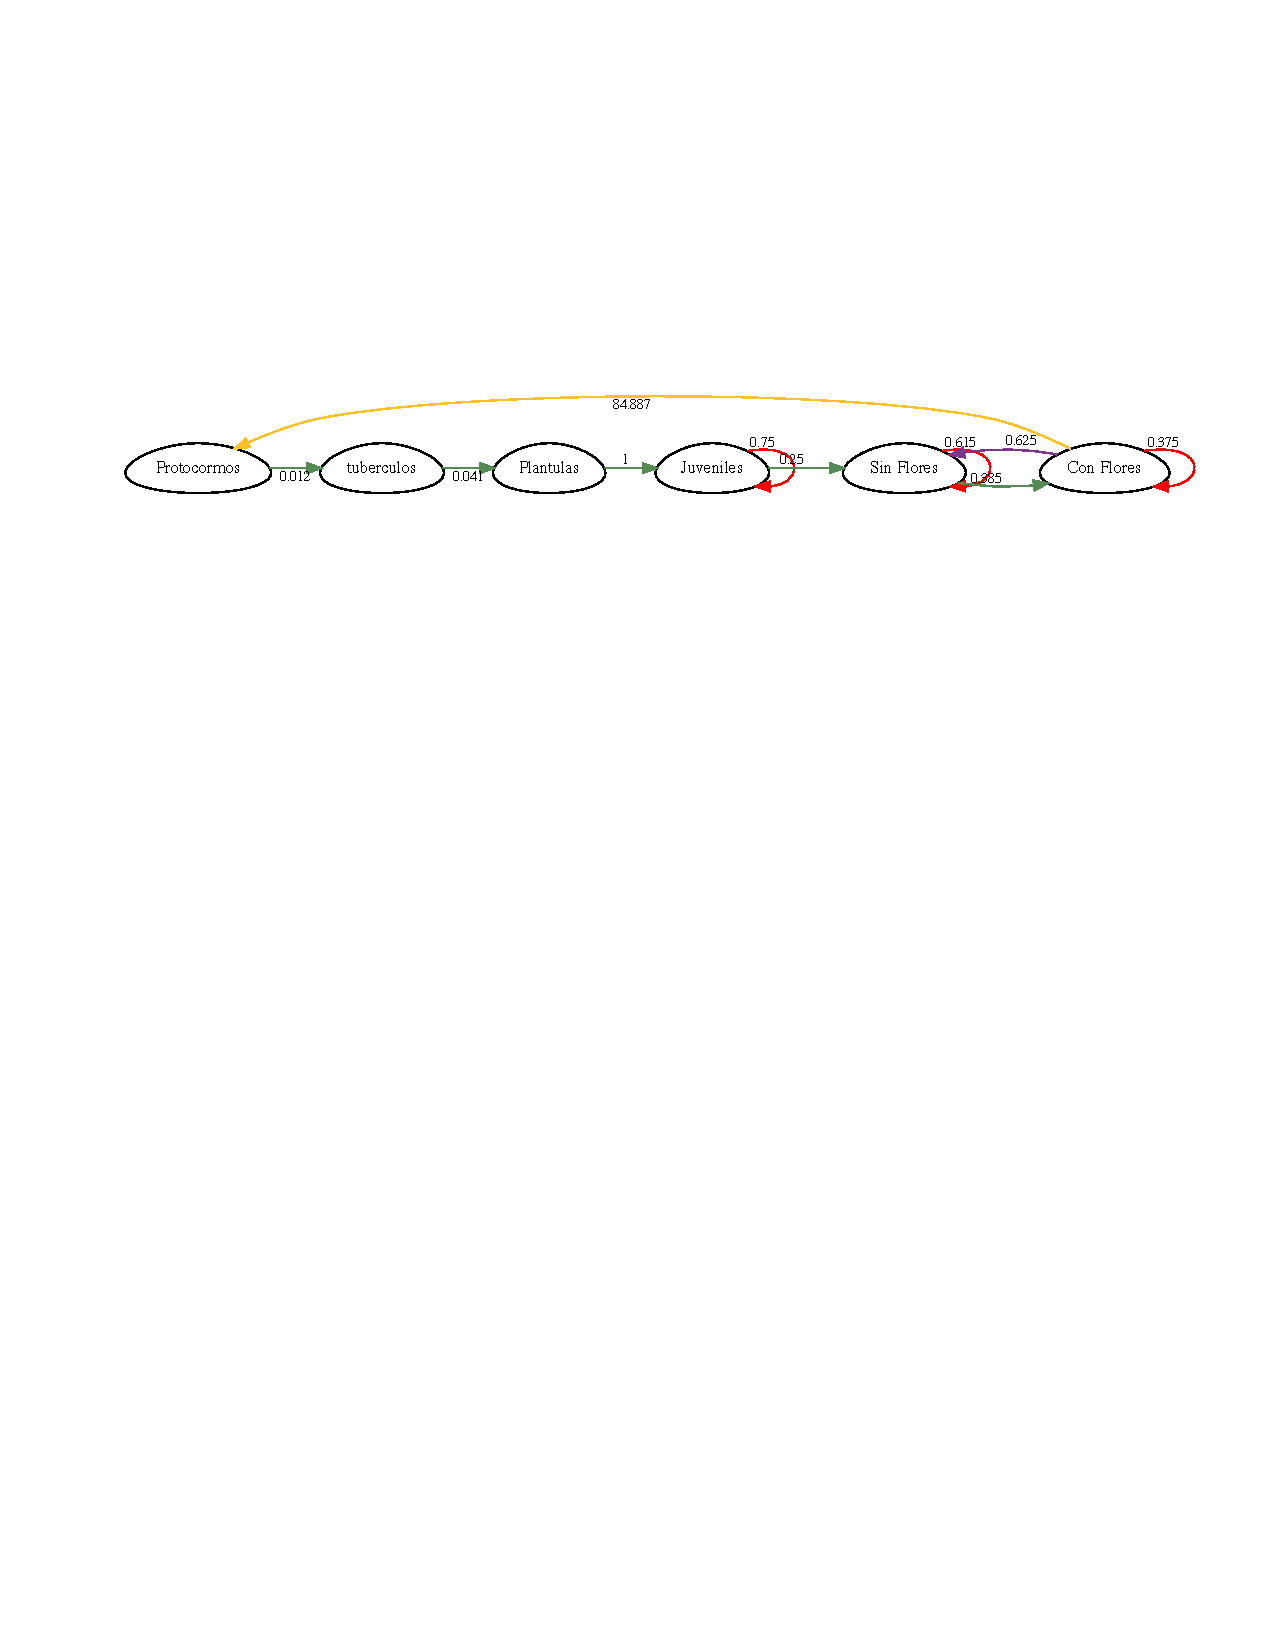
\includegraphics{103-Ciclos_de_Vida_files/figure-pdf/CV9_Os-1.pdf}

\begin{center}\rule{0.5\linewidth}{0.5pt}\end{center}

\subsection{Ejemplo de un ciclo de vida incompleto (y biologicamente
erroneos)}\label{ejemplo-de-un-ciclo-de-vida-incompleto-y-biologicamente-erroneos}

La importancia de este capítulo radica en reconocer la diferencia entre
la historia de vida real de un organismo y la información que se puede
recolectar en el campo. En los estudios poblacionales de orquídeas, dos
desafios en su investigación y muestreo son la dificultad, por un lado,
de rastrear y hacer una seguimiento de las semillas en el campo y, por
otro, el determinar los sitios adecuados para su germinación (sitios
seguros). Este segundo aspecto implica considerar la presencia de
micorrizas, cuya asociación con las semillas es determinante para su
germinación. Estas etapas tempranas en del ciclo de vida de las
orquídeas suelen estar rodeadas de gran incertidumbre, lo que limita los
análisis e interpretaciones de su evolución y conservación.

Además de los anteriores, existes otros problemas. La recolección de
datos en campo puede ser irreal en el contexto de historia de vida y la
base matemática del modelo representado. Para más detalles ver el
capitulo ``Impacto de datos sin sentidos''. A qué me refiero, en la
siguiente figura aparecen tres errores comunes durante la recolectan
datos de la historia de vida de una especie. El primero es que no hay
mortalidad de los individuos en una de las etapas (juveniles), el
segundo es que todos los individuos se mueren (plántulas) y el tercero
es que los individuos se mantienen en la misma etapa de desarrollo
(adultos) y no hay muerte. Dada la muerte de las plántulas, no hay
flecha que una este estado a otros estados. La falta de continuidad o
conexión entre las etapas del ciclo de vida son errores que ocurren
típicamente cuando el tamaño de muestra es pequeña o la probabilidad de
transición es rara o poco frecuente; por ejemplo, los árboles grandes no
fallecen. Estos son los tres errores típicos que a los que nos
enfrentamos cuando se lleva a cabo un análisis de dinámica poblacional
en especies con transiciones poco comunes.

\begin{verbatim}
file:////private/var/folders/3k/1ft37x9130vdbz21tw1497x40000gn/T/RtmpTIXuwN/file1061a39be8dfa/widget1061ad5b35b4.html screenshot completed
\end{verbatim}

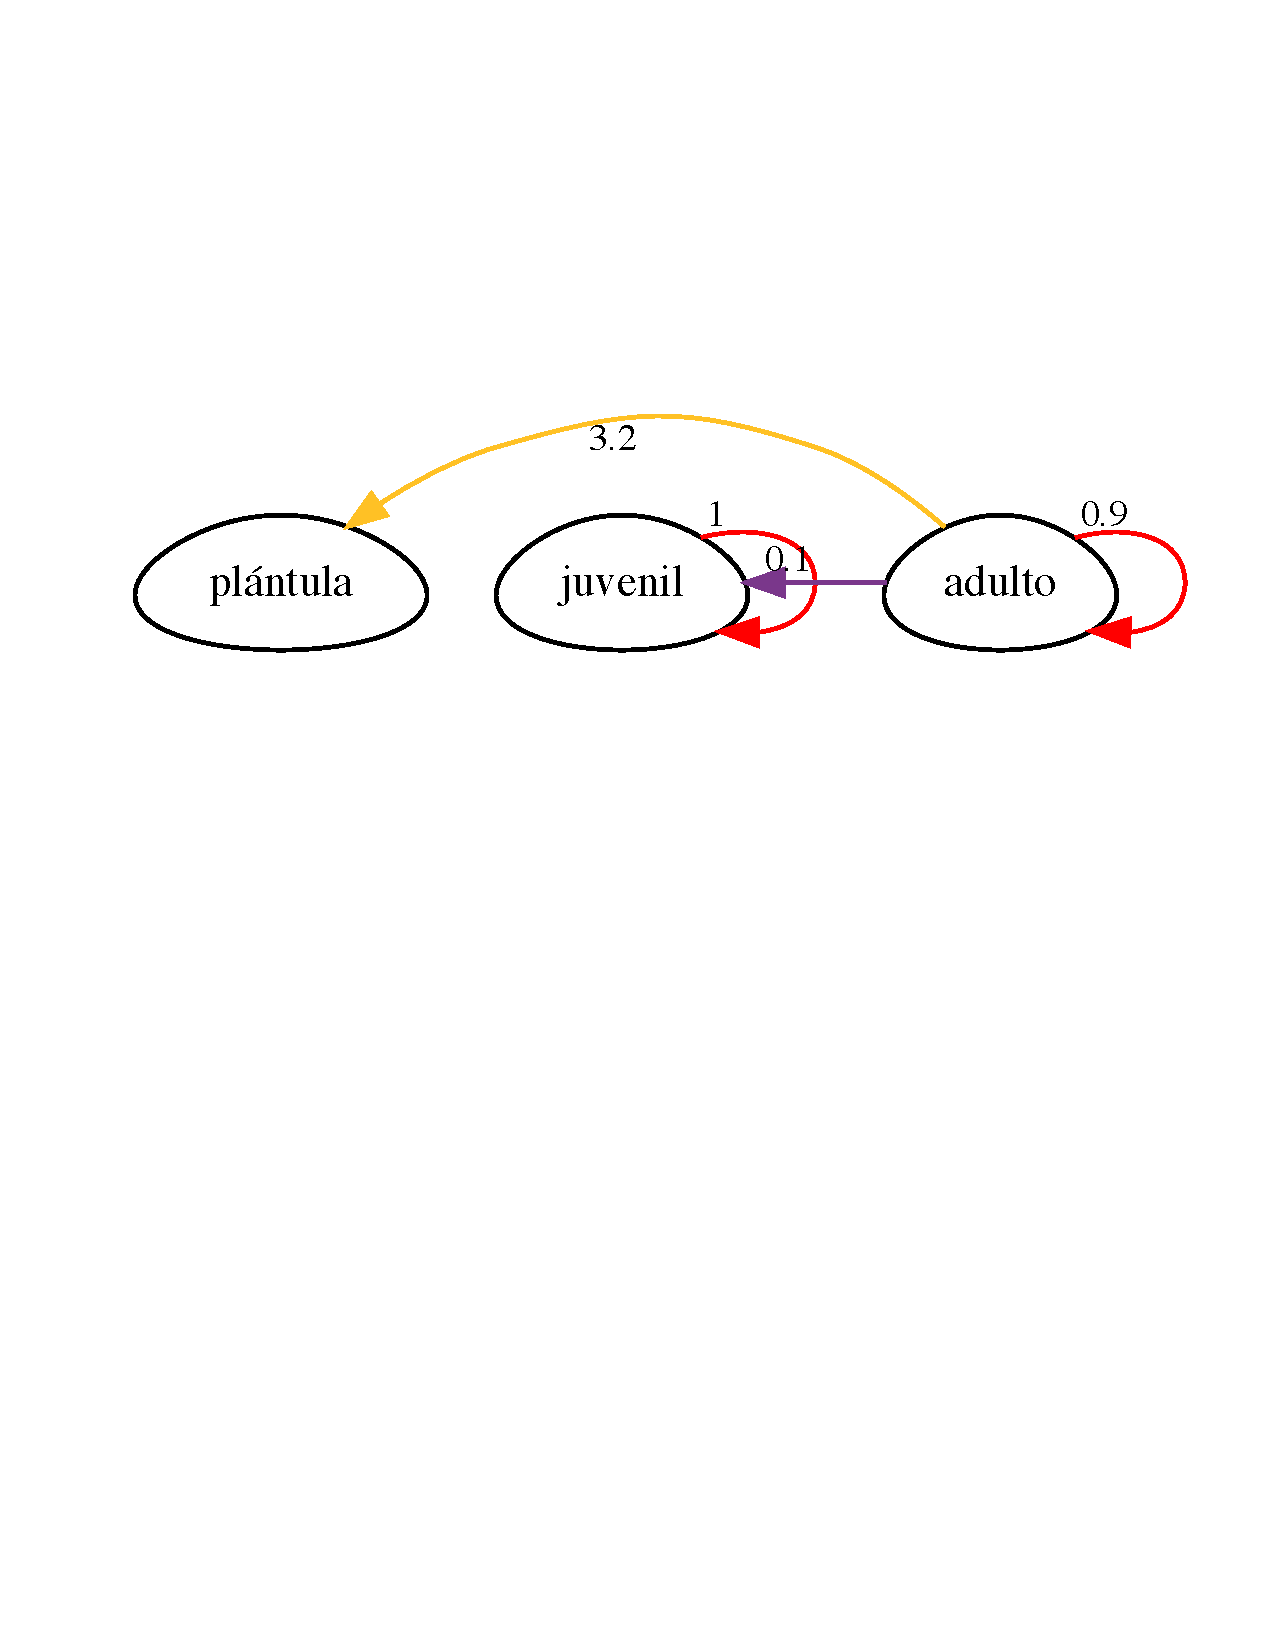
\includegraphics{103-Ciclos_de_Vida_files/figure-pdf/CV10-1.pdf}

\begin{center}\rule{0.5\linewidth}{0.5pt}\end{center}

\section{Ejemplo de un diagrama de un ciclo de vida usando el paquete
ggplot}\label{ejemplo-de-un-diagrama-de-un-ciclo-de-vida-usando-el-paquete-ggplot}

En la graficación del ciclo de vida podemos usar otro paquete de R
(Rage). La diferencia es que no se pueden cambiar los colores de las
líneas y los nodos (círculos que representan los estados de desarrollo).
Esta es una opción más sencilla para crear diagramas de ciclo de vida,
además de ser práctica para publicaciones donde no se necesita cambiar
los colores de las líneas y nodos.

\begin{Shaded}
\begin{Highlighting}[]
\FunctionTok{plot\_life\_cycle}\NormalTok{(matA, }\AttributeTok{stages=}\FunctionTok{c}\NormalTok{(}\StringTok{"semillas"}\NormalTok{, }\StringTok{"plantulas"}\NormalTok{, }\StringTok{"adultos"}\NormalTok{),}\AttributeTok{fontsize =} \FloatTok{0.1}\NormalTok{)}
\end{Highlighting}
\end{Shaded}

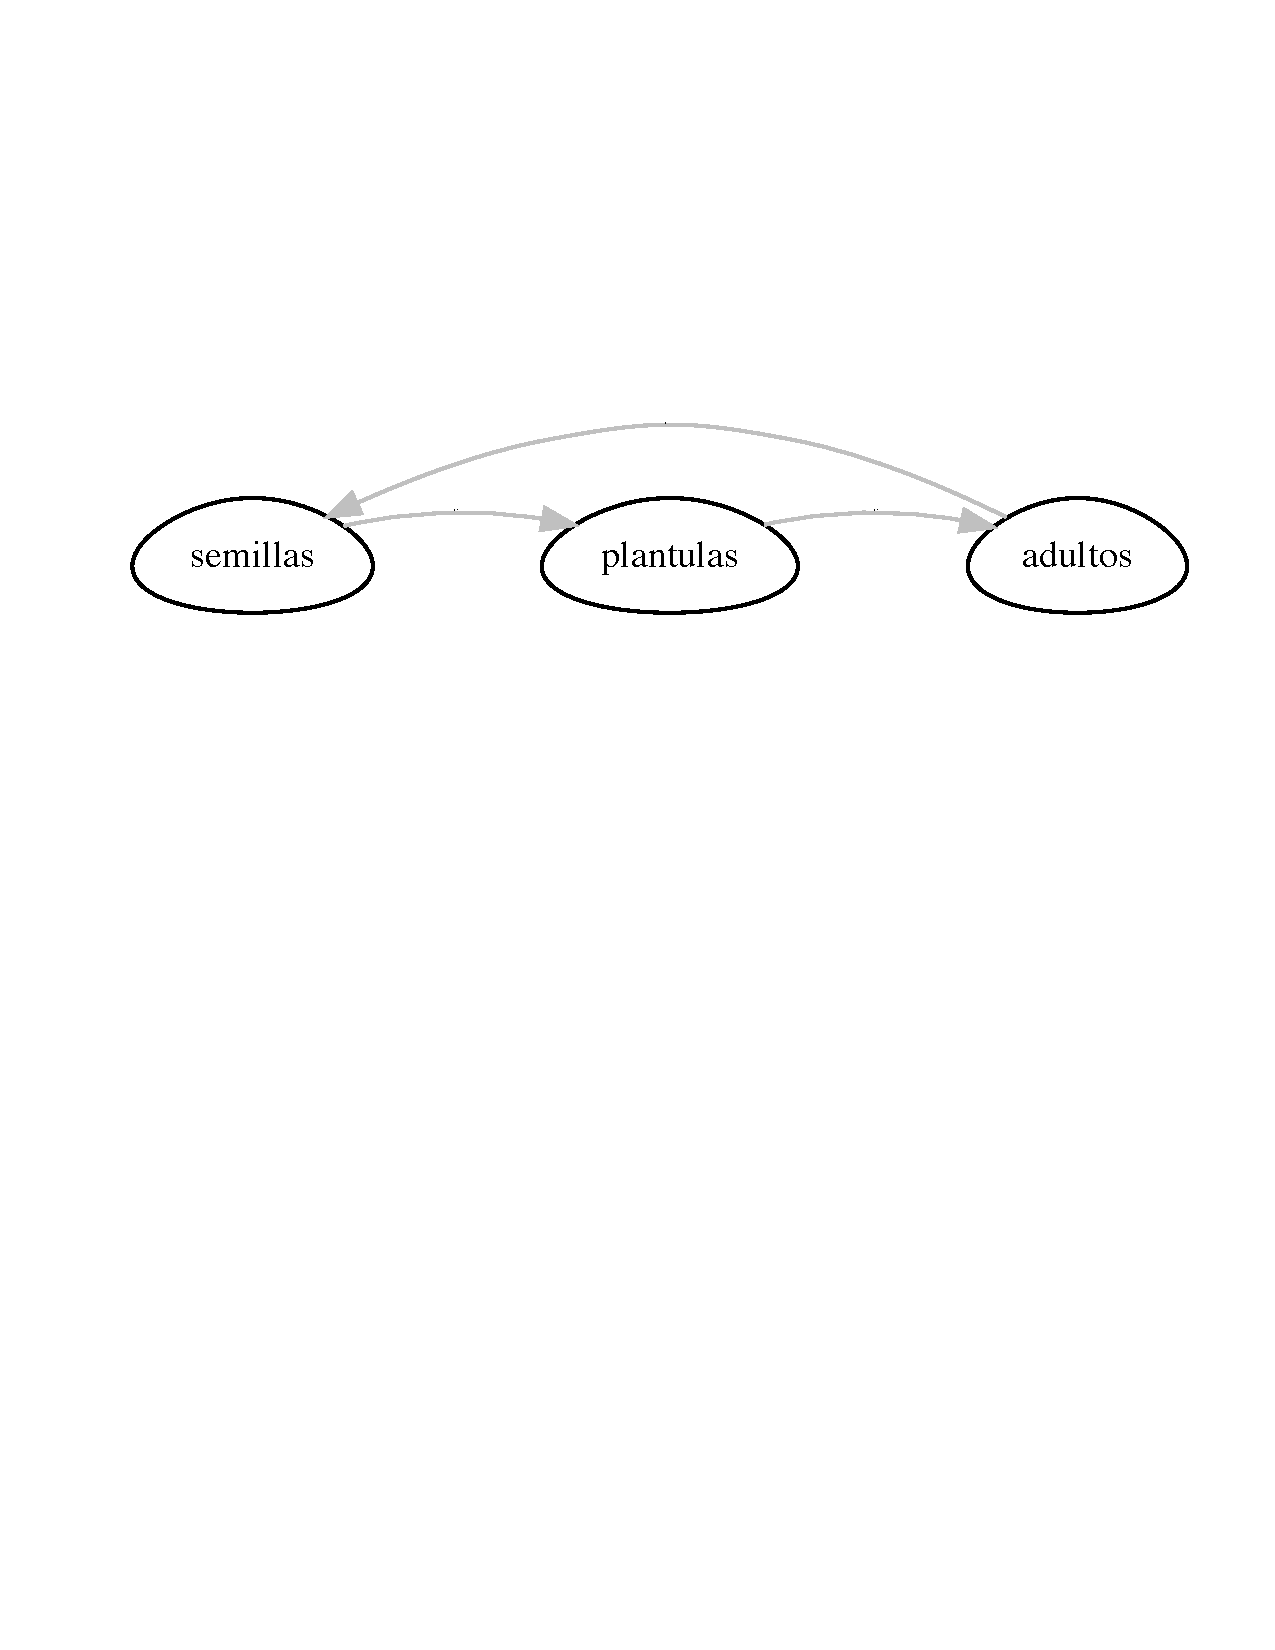
\includegraphics{103-Ciclos_de_Vida_files/figure-pdf/CV11-1.pdf}

\begin{Shaded}
\begin{Highlighting}[]
\DocumentationTok{\#\# Code for color coding figure}
\CommentTok{\# http://rich{-}iannone.github.io/DiagrammeR/}
\end{Highlighting}
\end{Shaded}

Revision:

RLT Sept 14, 2024

RLT May, 25, 2025

Mariana Nov 20, 2025

\phantomsection\label{refs}
\begin{CSLReferences}{1}{0}
\bibitem[\citeproctext]{ref-coates2006effects}
Coates F, Lunt ID, Tremblay R. 2006. Effects of disturbance on
population dynamics of the threatened orchid \emph{{P}rasophyllum
{c}orrectum} DL jones and implications for grassland management in
south-eastern {A}ustralia. \emph{Biological Conservation} 129:59--69.

\bibitem[\citeproctext]{ref-hernandez1992dinamica}
Hernández-Apolinar M. 1992. Din{á}mica poblacional de \emph{{L}aelia
{s}peciosa} (HBK) schltr. ({O}rchidaceae). Master's thesis Thesis.
Mexico City, Mexico: Faculdad de Ciencias, UNAM.

\bibitem[\citeproctext]{ref-jacquemyn2010seed}
Jacquemyn H, Brys R, Jongejans E. 2010. Seed limitation restricts
population growth in shaded populations of a perennial woodland orchid.
\emph{Ecology} 91:119--129.

\bibitem[\citeproctext]{ref-jakalaniemi2011orchids}
Jäkäläniemi A, Crone EE, Närhi P, Tuomi J. 2011. Orchids do not pay
costs at emergence for prolonged dormancy. \emph{Ecology} 92:1538--1543.

\bibitem[\citeproctext]{ref-raventos2018comparison}
Raventós J, Garcı́a-González A, Riverón-Giró FB, Damon A. 2018.
Comparison of transient and asymptotic perturbation analyses of three
epiphytic orchid species growing in coffee plantations in {M}exico:
Effect on conservation decisions. \emph{Plant Ecology \& Diversity}
11:133--145.

\bibitem[\citeproctext]{ref-shefferson2014life}
Shefferson RP, Warren RJ, Pulliam HR. 2014. Life-history costs make
perfect sprouting maladaptive in two herbaceous perennials.
\emph{Journal of Ecology} 102:1318--1328.

\bibitem[\citeproctext]{ref-tremblay2009dormancy}
Tremblay R, Perez M, Larcombe M, Brown A, Quarmby J, Bickerton D, French
G, Bould A. 2009. Dormancy in \emph{{C}aladenia}: A {B}ayesian approach
to evaluating latency. \emph{Australian Journal of Botany} 57:340--350.

\bibitem[\citeproctext]{ref-waite1991effects}
Waite S, Hutchings M. 1991. The effects of different management regimes
on the population dynamics of \emph{{O}phrys {s}phegodes}: Analysis and
description using matrix models. In: Wells TCE, Willems JH eds.
\emph{Population ecology of terrestrial orchids}. SPB Academic
Publishing bv, The Hague, 161--175.

\end{CSLReferences}


\backmatter


\end{document}
